\chapter{Intégration des objets connectés}
%\markboth{Chapitre 4}{Intégration des objets connectés} %pour afficher l'entete
% \addcontentsline{toc}{chapter}{Chapitre 4 : Intégration des objets connectés}

\section{Introduction}

L'intégration des objets connectés est un élément clé pour une infrastructure informatique moderne et efficace. Dans ce dernier chapitre, nous allons explorer les différentes étapes de l'intégration des objets connectés dans notre infrastructure existante. \\

Les objets connectés sont des dispositifs électroniques qui peuvent communiquer entre eux et avec des systèmes informatiques, et sont capables de collecter et d'analyser des données en temps réel. \\

Ils jouent un rôle important dans la création de systèmes intelligents et autonomes, qui peuvent améliorer l'efficacité, la sécurité et la qualité de vie dans de nombreux domaines. \\

Dans ce chapitre, nous examinerons les différentes technologies et protocoles utilisés pour l'intégration des objets connectés, ainsi que les défis et les opportunités qu'elle présente. \\

Nous décrirons également les différentes étapes du processus d'intégration, de la sélection des dispositifs appropriés à leur installation, leur configuration et leur maintenance. Enfin, nous présenterons quelques exemples d'applications pratiques de l'intégration des objets connectés dans différents domaines, tels que l'agriculture, la santé, l'industrie et le transport. \\







\section{Objets Connectés}

Les objets connectés, également connus sous le nom d'Internet des objets (IoT), font référence à des appareils physiques qui sont connectés à Internet et peuvent échanger des données avec d'autres appareils ou systèmes. \\

 Les objets connectés sont souvent équipés de capteurs, de logiciels et d'autres technologies permettant de collecter et de communiquer des données en temps réel. Ces données peuvent être utilisées pour améliorer l'efficacité, la productivité et la sécurité dans un large éventail de domaines, tels que la santé, les transports, l'agriculture, l'industrie manufacturière, les villes intelligentes, les maisons intelligentes, etc. \\

\begin{figure}[H]
 \centering
    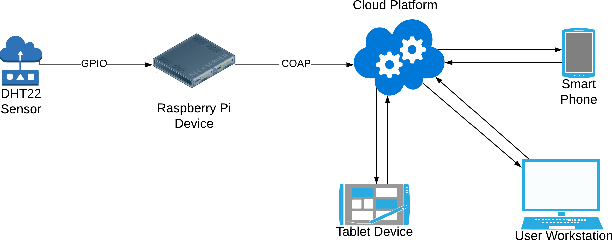
\includegraphics[width=15cm]{Images/IoT-Topo2.png}
    \caption{Topologie IoT}
    \label{Chap4.2.1}
\end{figure}    
\smallskip


\subsection{Imprimantes}

\begin{figure}[H]
 \centering
    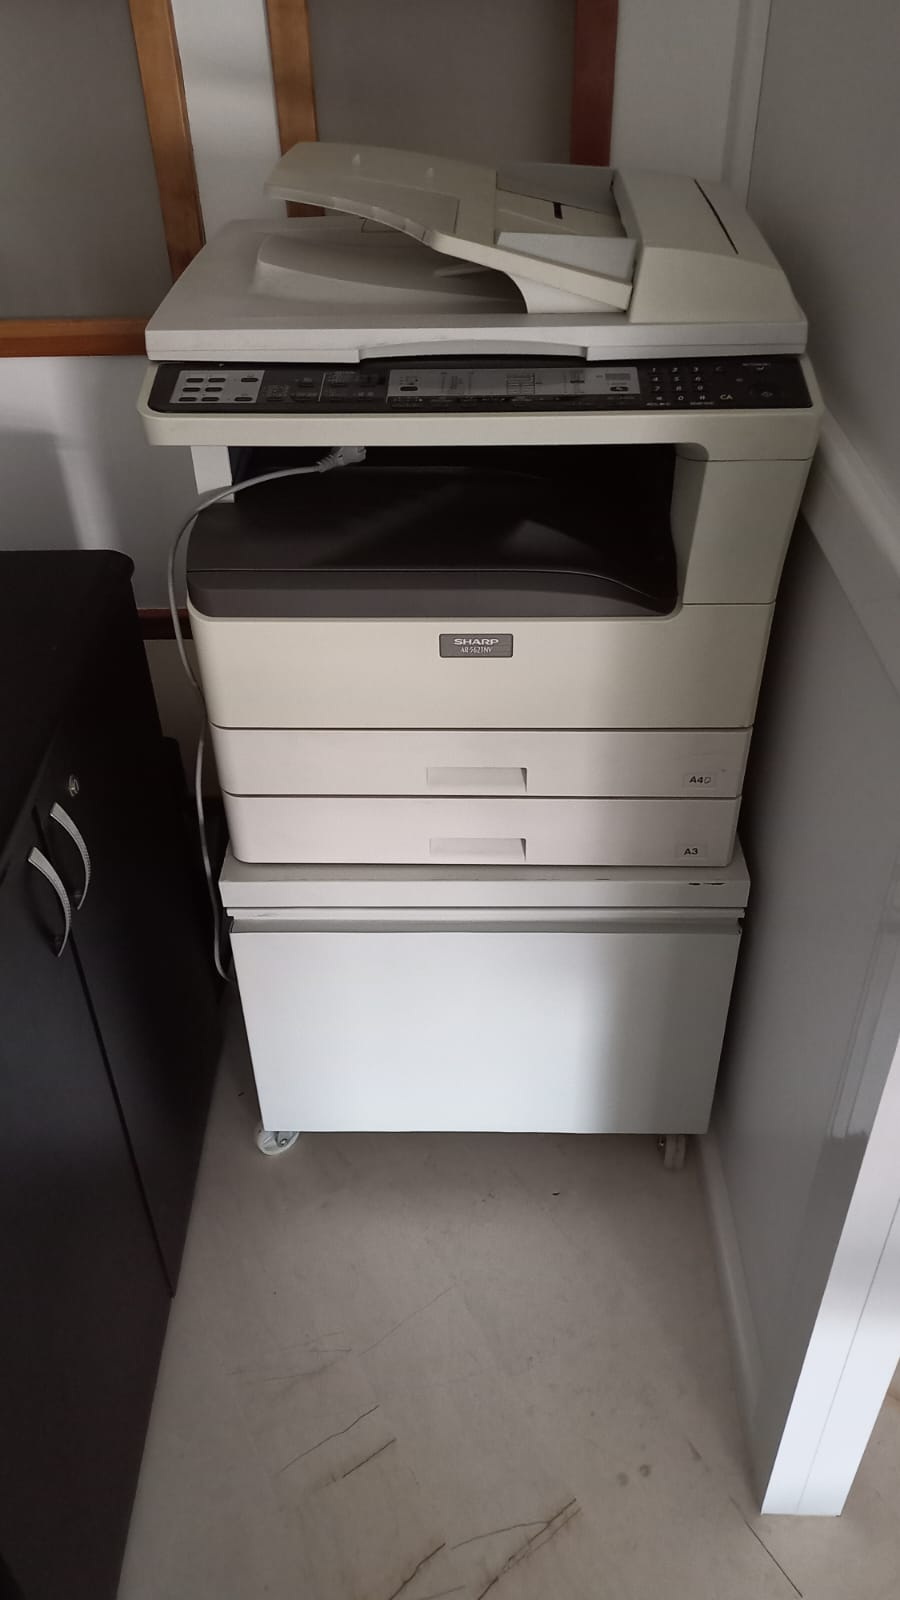
\includegraphics[width=10cm,height=10cm]{Images/BRades-Imprimante.jpg}
    \caption{Imprimante de l'entreprise}
    \label{Chap4.2.2}
\end{figure}    
\smallskip

La plupart des imprimantes appartenant à l'entreprise sont équipées d'une carte réseau permettant leur intégration au réseau. Toutefois, celles qui n'en disposent pas utilisent une carte intégrée pour se connecter. \\

\subsection{Camera de Surveillance}

\begin{figure}[H]
 \centering
    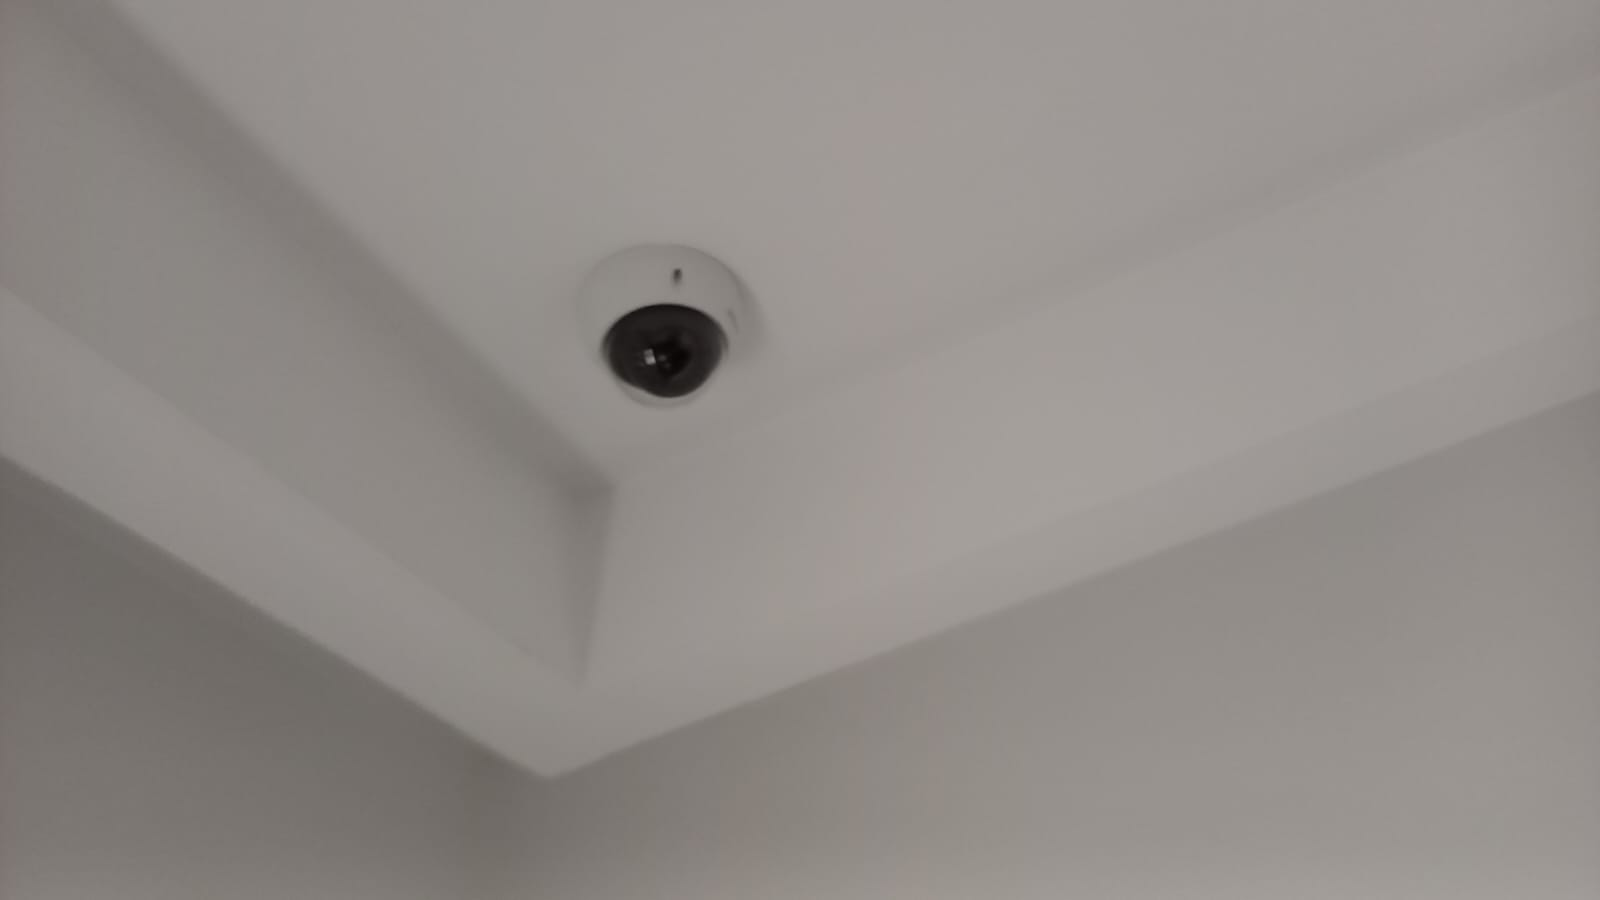
\includegraphics[width=10cm]{Images/BRades-CCTV.jpg}
    \caption{Camera Dahua de l'entreprise}
    \label{Chap4.2.3}
\end{figure}    
\smallskip




Pour connecter les caméras de surveillance au réseau de l'entreprise, nous commencerons par configurer chaque caméra afin qu'elle obtienne une adresse IP unique et qu'elle soit reconnue sur le réseau. Ensuite, nous utiliserons un NVR pour stocker les enregistrements vidéo en continu et gérer les flux provenant des caméras. Pour faciliter l'accès aux flux vidéo des caméras, nous installerons le logiciel SmartPSS sur les ordinateurs des directeurs. \\


\begin{figure}[H]
 \centering
    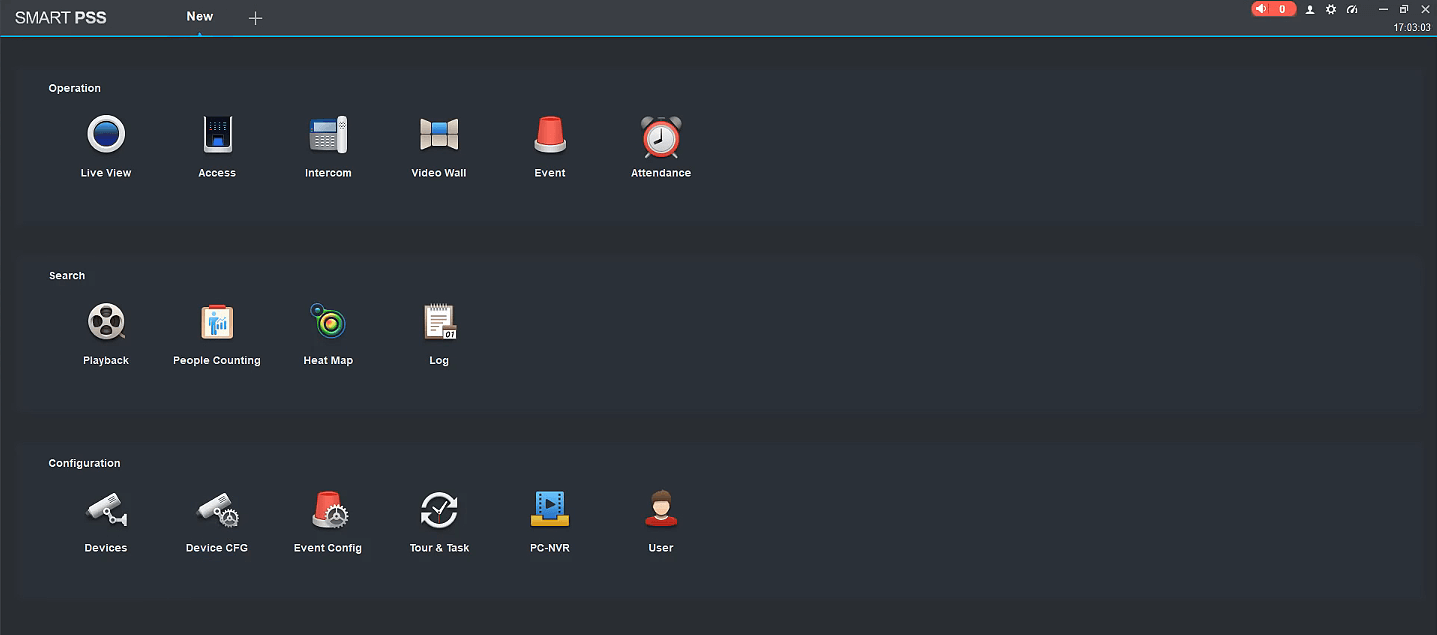
\includegraphics[width=15cm]{Images/SmartPSS-Logiciel.png}
    \caption{Logiciel SmartPSS}
    \label{Chap4.2.4}
\end{figure}    
\smallskip

SmartPSS est un logiciel créé par Dahua, un leader mondial dans le domaine des systèmes de vidéosurveillance. Il permet une gestion centralisée des caméras, ainsi que l'enregistrement et la lecture des vidéos enregistrées. Ce logiciel est convivial et offre une interface intuitive pour faciliter l'utilisation par les utilisateurs finaux. \\





\subsection{Machine de Pointage}

\begin{figure}[H]
 \centering
    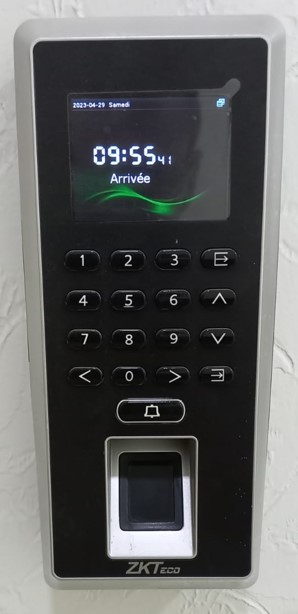
\includegraphics[height=14cm,width=8cm]{Images/BRades-Pointage.jpg}
    \caption{Machine de pointage ZKTeco}
    \label{Chap4.2.5}
\end{figure}    
\smallskip

Pour intégrer les machines de pointage dans le réseau de l'entreprise et les contrôler, nous utiliserons le logiciel ZKAccess développé par ZKTeco. Ce logiciel permettra d'assurer la communication entre les machines et le réseau et ainsi permettre un accès facile et sécurisé aux données de pointage. \\

\begin{figure}[H]
 \centering
    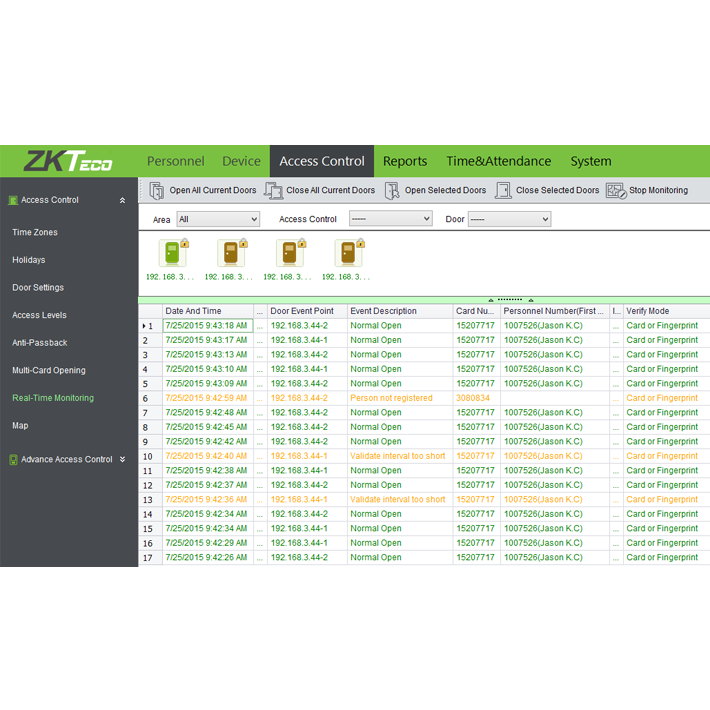
\includegraphics[width=15cm]{Images/ZKAccess3-Logiciel.png}
    \caption{Logiciel ZKAccess 3.5}
    \label{Chap4.2.6}
\end{figure}    
\smallskip

\subsection{Les Lampes et le Theromstat}

L'intégration des objets connectés (IoT) dans les foyers a connu une croissance significative ces dernières années. Selon Statista, en 2020, le nombre d'appareils IoT connectés dans le monde a atteint 26,66 milliards, et ce chiffre devrait augmenter à 75,44 milliards d'ici 2025. Les dispositifs IoT incluent une variété d'objets connectés tels que les caméras de surveillance, les machines de pointage, et les lampes intelligentes (smart blubs). \\

Les smart blubs sont l'une des applications les plus courantes de l'IoT dans les foyers. Selon un rapport de Grand View Research, le marché des lampes intelligentes devrait atteindre une valeur de 38,68 milliards de dollars d'ici 2027, avec un taux de croissance annuel composé de 20,8\%. Bien que la plupart des lampes ne soient pas des smart blubs, elles peuvent être connectées à notre réseau grâce à des cartes IoT comme Raspberry Pi ou Arduino. \cite{gazis2021iot}\\

\begin{figure}[H]
 \centering
    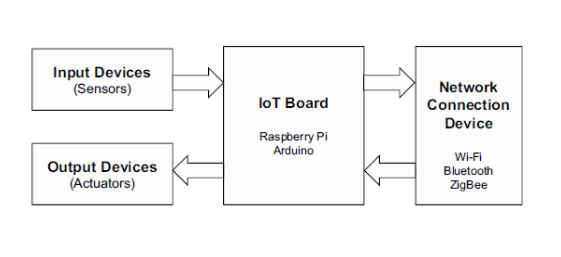
\includegraphics[width=15cm]{Images/IoT-Topo.png}
    \caption{Topologie IoT 2}
    \label{Chap4.2.8}
\end{figure}    
\smallskip

Pour répondre à la demande de l'entreprise d'avoir un SmartHome et de contrôler les lampes à distance, l'utilisation d'une carte IoT est essentielle. Par exemple, en utilisant Raspberry Pi ou Arduino, il est possible de connecter les lampes à notre réseau et de les contrôler à distance. \\

Cela permettrait à l'entreprise de gérer les lumières de manière centralisée et d'optimiser l'utilisation de l'énergie, ce qui peut conduire à des économies significatives sur les coûts d'énergie. En fin de compte, l'intégration d'objets connectés tels que les lampes intelligentes dans le réseau de l'entreprise peut contribuer à améliorer l'efficacité opérationnelle et la qualité de vie des employés. \\




\section{Solution avec Raspberry Pi}

Face à ce défi, notre choix s'est porté sur l'utilisation de Raspberry Pi pour connecter les lampes à notre réseau. Raspberry Pi est une carte informatique très performante et polyvalente qui peut être utilisée pour de nombreux projets IoT. \cite{richardson2012getting} \\

Nous avons décidé d'utiliser Node-RED, un outil de programmation visuel pour créer une application permettant de contrôler les lampes à distance. Node-RED est une plateforme open source qui facilite la création de flux de données entre différents objets connectés. \cite{lekic2018iot} \\

En utilisant Raspberry Pi et Node-RED, nous sommes en mesure de créer une solution robuste et évolutive pour connecter les lampes à notre réseau. Cette solution nous permet de contrôler les lampes à distance à partir de n'importe quel appareil connecté à notre réseau. \\


\subsection{Installation Raspberry Pi OS}

Avant tout Il faut installé l'OS Debian du Raspberry Pi sur une carte mémoire et l'insérer dans notre carte électronique 



Pour commencer, nous devons installer l'OS Debian spécifique au Raspberry Pi sur une carte mémoire. Cette carte mémoire sera ensuite insérée dans notre carte électronique Raspberry Pi pour démarrer le système. \\

L'installation du Raspberry Pi OS est une étape essentielle pour configurer notre infrastructure. Cette distribution d'exploitation est spécialement conçue pour le Raspberry Pi et offre une compatibilité optimale avec ses fonctionnalités et ses composants matériels.


Une fois que nous avons téléchargé le Raspberry Pi Imager depuis le site officiel, nous utilisons cet outil comme Etcher pour graver sur notre carte mémoire. 


\begin{figure}[H]
 \centering
    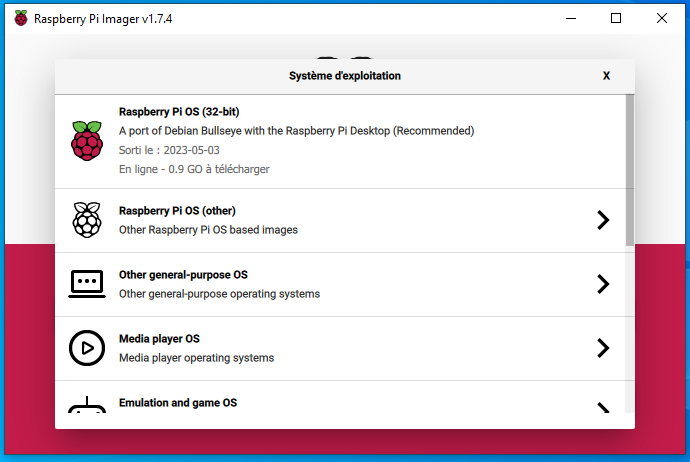
\includegraphics[width=15cm]{Images/RaspberryPiOSInstall1.png}
    \caption{Installation du Raspberry Pi OS}
    \label{Chap4.3.1}
\end{figure}    
\smallskip

Une fois que l'image est gravée sur la carte mémoire, nous insérons celle-ci dans le slot prévu sur notre carte électronique Raspberry Pi. Cela permettra de démarrer le Raspberry Pi et d'accéder à l'interface utilisateur du système d'exploitation. \\

Une fois le Raspberry Pi OS démarré, nous pourrons effectuer les configurations supplémentaires nécessaires pour intégrer les objets connectés à notre infrastructure. Ces configurations peuvent inclure la connexion au réseau, l'installation de logiciels supplémentaires, et la personnalisation des paramètres en fonction de nos besoins spécifiques. \\

En résumé, l'installation du Raspberry Pi OS sur une carte mémoire et son insertion dans notre carte électronique Raspberry Pi constituent la première étape pour mettre en place notre infrastructure et intégrer les objets connectés. Cette étape est cruciale pour assurer la compatibilité et la stabilité de notre système. \\



\subsection{Installation Node-RED}


Après avoir préparé le Raspberry Pi, nous procédons à l'installation de Node-RED sur la carte à l'aide du script bash officiel disponible sur le site de Node-RED, comme illustré dans la figure suivante. \\



\begin{figure}[H]
 \centering
    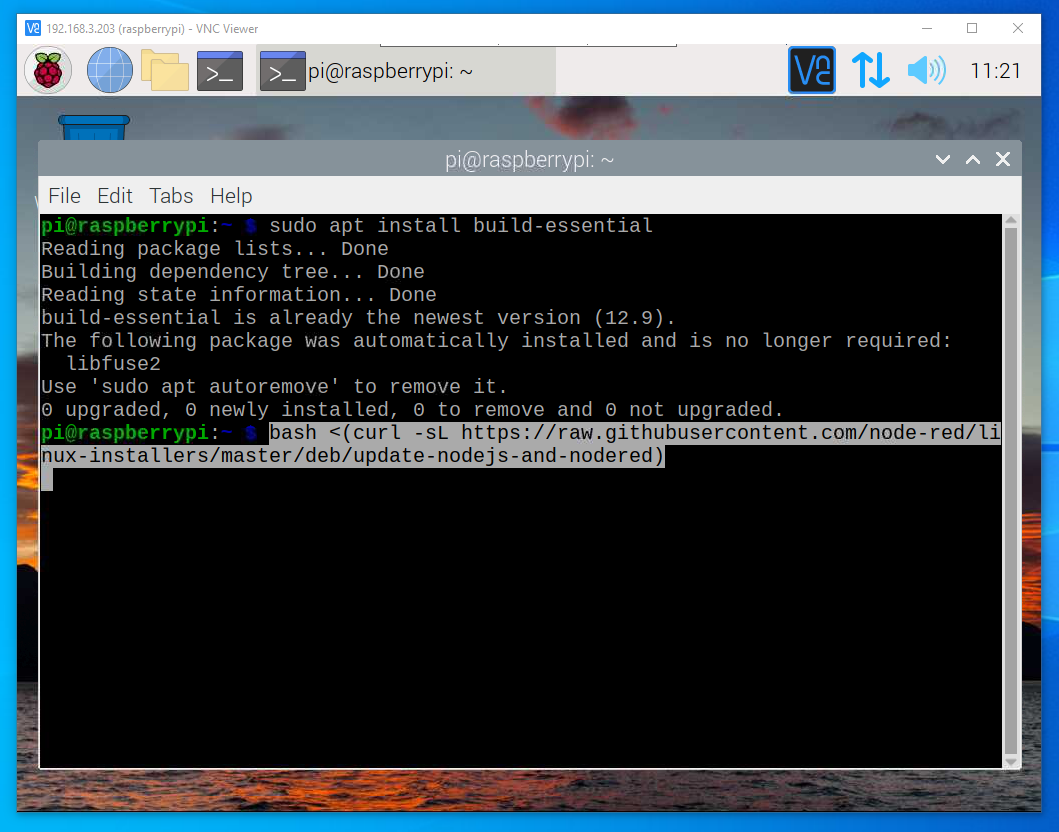
\includegraphics[width=15cm]{Images/NodeRedInstall1.png}
    \caption{Installation du Node-RED avec le Script Officiel Bash}
    \label{Chap4.3.2}
\end{figure}    
\smallskip

Ce script effectue une série d'étapes, telles que l'arrêt de Node-RED, la suppression des anciennes versions de Node-RED et de Node.js, l'installation de Node.js pour Armv6, la purification du cache npm, l'installation de Node-RED Core, le déplacement des nœuds globaux vers un emplacement local, la reconstruction des nœuds existants, l'installation de nœuds supplémentaires spécifiques à Raspberry Pi, l'ajout de commandes raccourcies et la mise à jour du script systemd. \\


\begin{figure}[H]
 \centering
    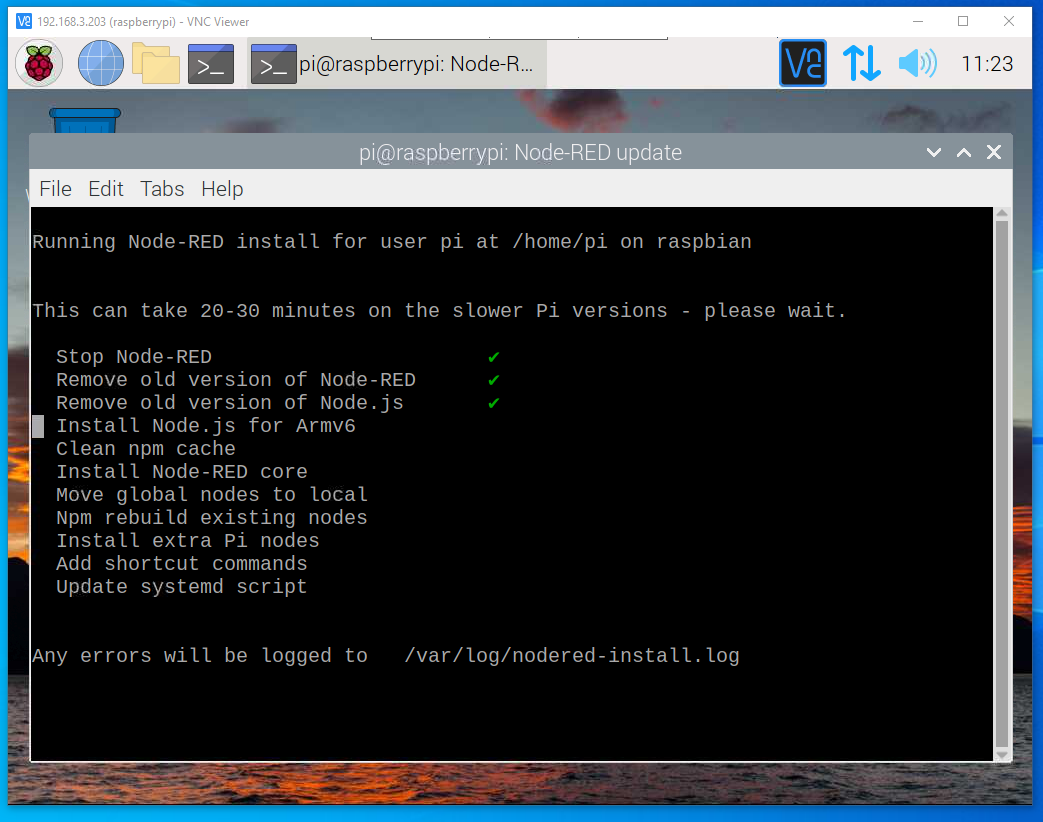
\includegraphics[width=13cm]{Images/NodeRedInstall2.png}
    \caption{En cours d'Installation du Node-RED}
    \label{Chap4.3.3}
\end{figure}    
\smallskip

\begin{figure}[H]
 \centering
    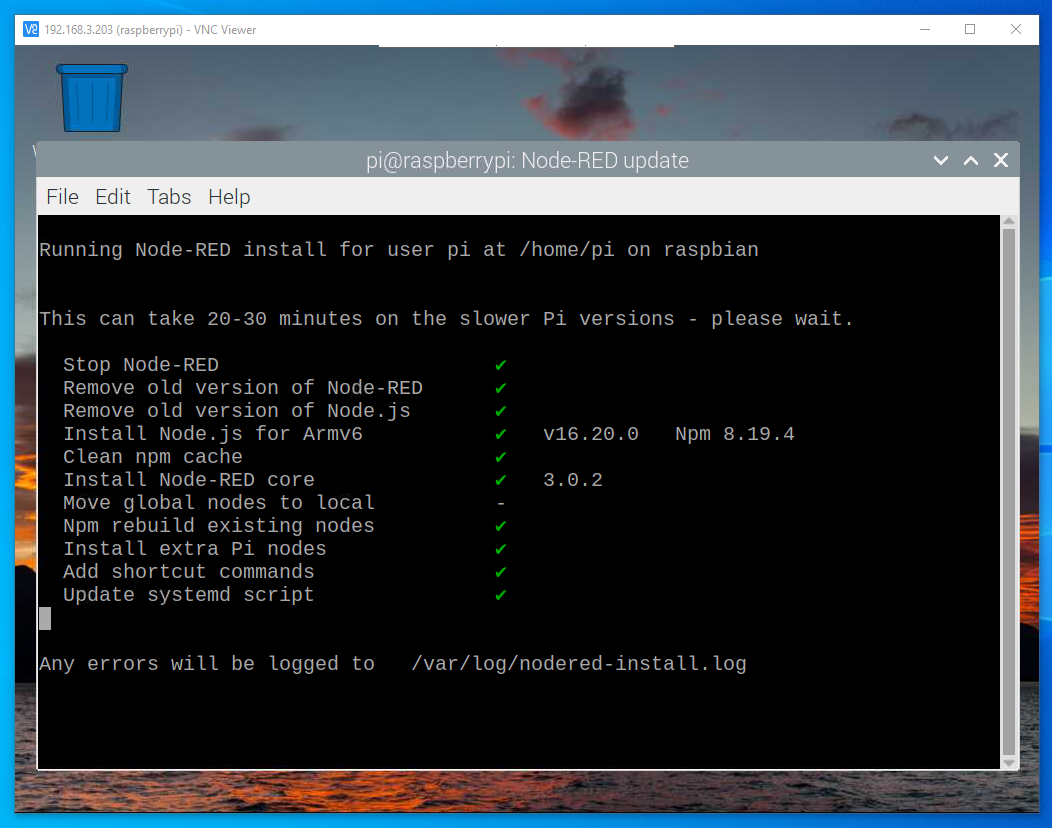
\includegraphics[width=13cm]{Images/NodeRedInstall3.png}
    \caption{En cours d'Installation du Node-RED}
    \label{Chap4.3.4}
\end{figure}    
\smallskip


Une fois l'installation terminée, nous pouvons démarrer Node-RED en utilisant la commande "node-red-start". Le résultat final du démarrage est illustré dans la figure suivante. \\


\begin{figure}[H]
 \centering
    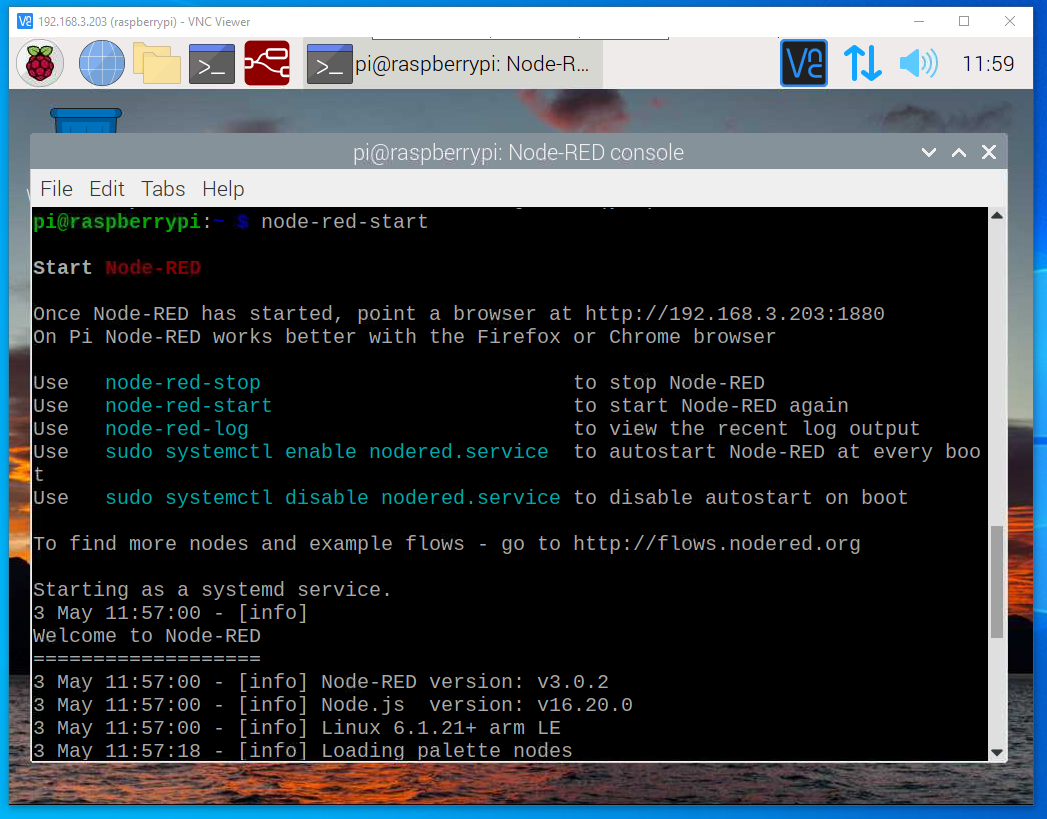
\includegraphics[width=15cm]{Images/NodeRedStart1.png}
    \caption{Le démarrage du Node-RED}
    \label{Chap4.3.5}
\end{figure}    
\smallskip


Node-RED est maintenant installé et opérationnel sur notre Raspberry Pi, prêt à être utilisé pour créer des flux et interagir avec les objets connectés de notre infrastructure. \\



\subsection{Préparation de Node-RED}

Pour accéder à Node-RED via le réseau, vous pouvez utiliser l'adresse IP de votre Raspberry Pi et le port 1880/ui. Voici à quoi ressemble notre première interface Node-RED :

\begin{figure}[H]
\centering
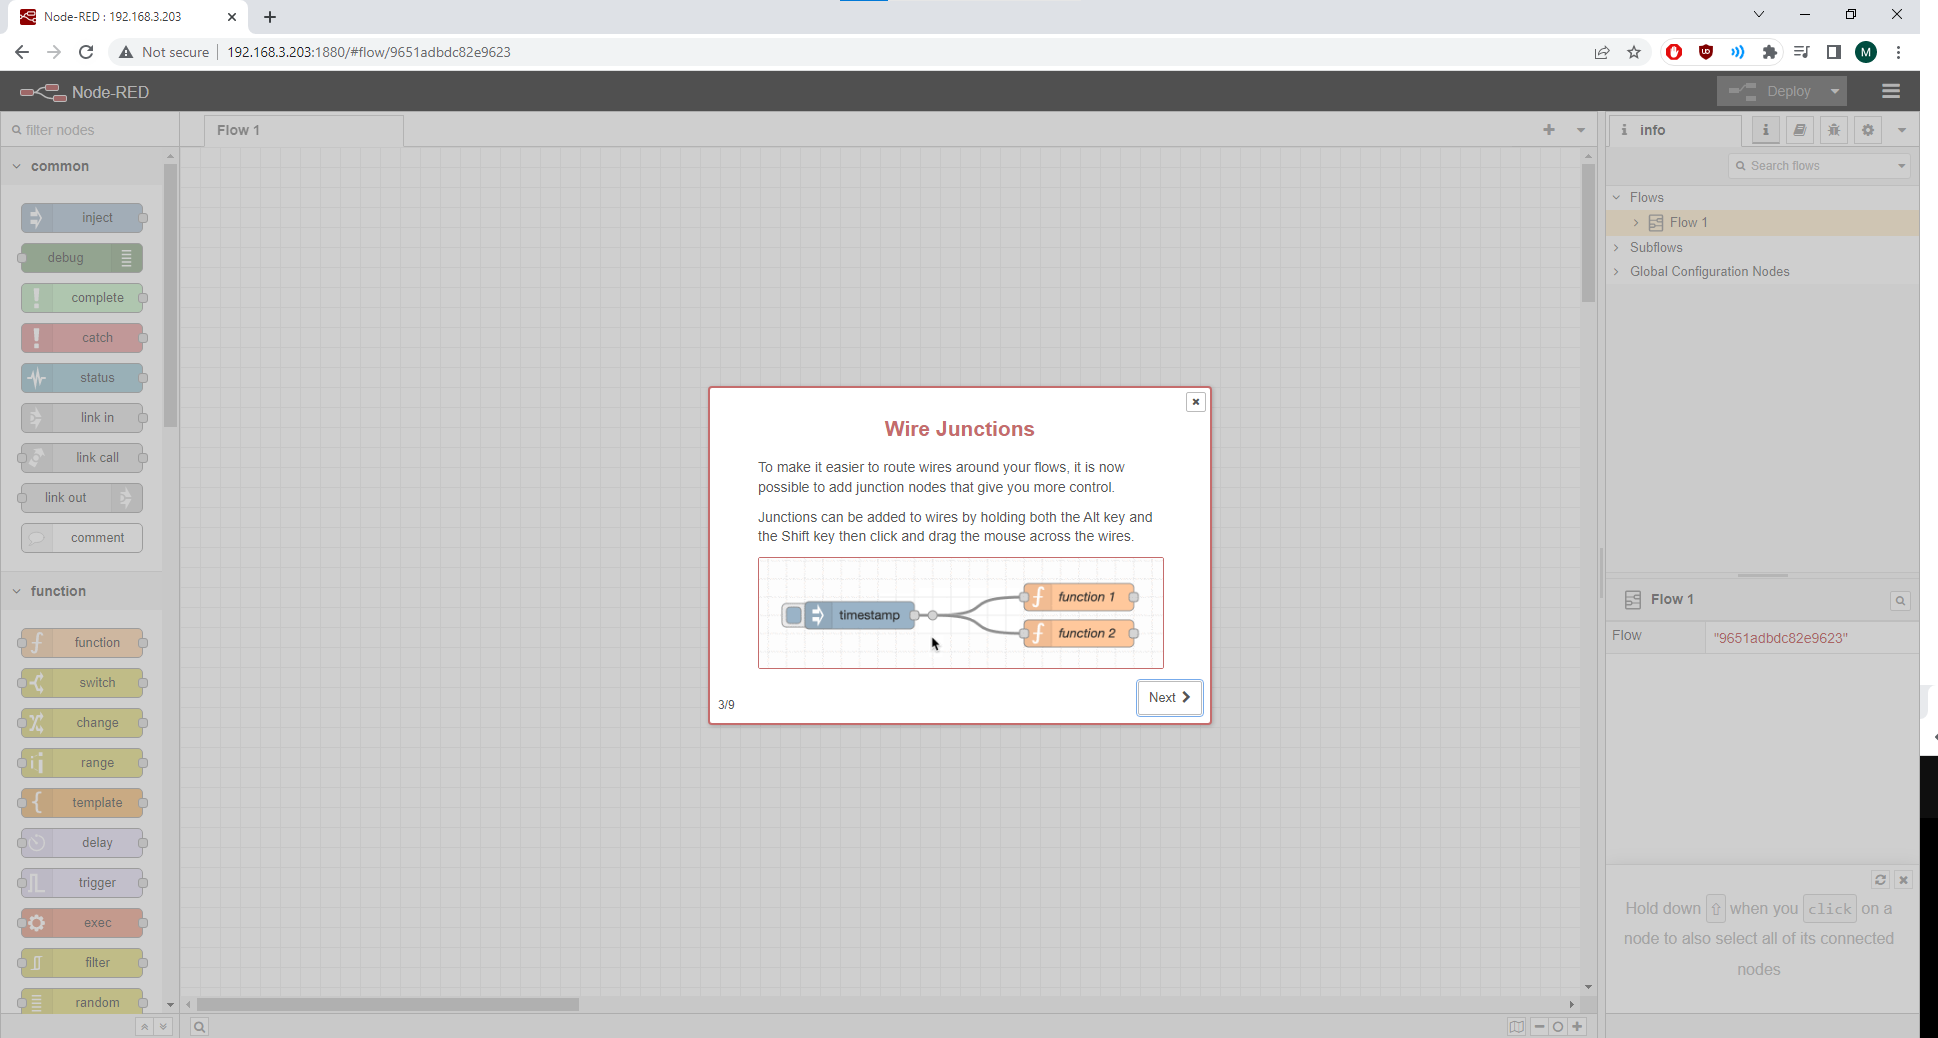
\includegraphics[width=15cm]{Images/NodeRedInterface.png}
\caption{Interface Node-RED}
\label{Chap4.3.6}
\end{figure}

Dans la figure \ref{Chap4.3.6}, nous pouvons observer l'interface de Node-RED, où nous pouvons développer notre projet en utilisant des nœuds et des connexions pour créer des flux de données.

Pour notre projet, nous devons installer quelques nœuds supplémentaires. Par exemple, le "dashboard" pour créer une interface graphique conviviale permettant d'interagir avec le projet, et le nœud DHT11 pour détecter notre thermostat dans Node-RED.

\begin{figure}[H]
\centering
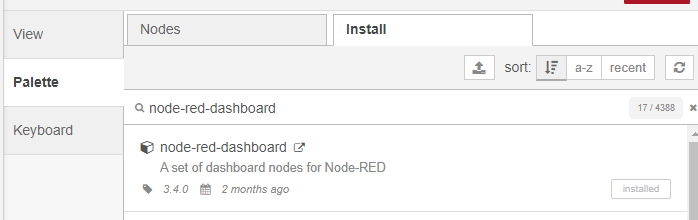
\includegraphics[width=15cm]{Images/Node-Red-Dashboard-Installed.png}
\caption{Installation du dashboard Node-RED}
\label{Chap4.3.7}
\end{figure}

La figure \ref{Chap4.3.7} montre le processus d'installation du nœud "dashboard" dans Node-RED, qui permet de créer des tableaux de bord interactifs pour contrôler et visualiser les données de notre projet.

\begin{figure}[H]
\centering
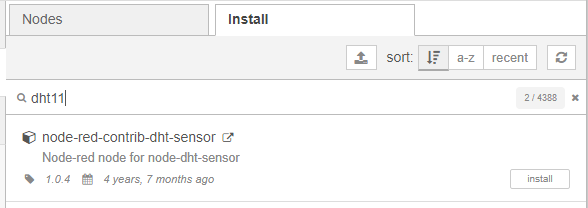
\includegraphics[width=15cm]{Images/DHT11-Node-Red-Install.png}
\caption{Installation du nœud DHT11 dans Node-RED}
\label{Chap4.3.8}
\end{figure}

Dans la figure \ref{Chap4.3.8}, nous avons installé le nœud DHT11 dans Node-RED, qui nous permet de capturer les données de notre capteur de température et d'humidité.

Ces différentes figures illustrent la préparation de Node-RED et l'installation des nœuds nécessaires pour notre projet. Ils servent de base à la réalisation de notre système de surveillance et de contrôle.


\subsection{Sécurité de Node-RED}

Pour sécuriser Node-RED, nous utilisons une méthode fournie par le site officiel de Node-RED, qui nous permet de créer des mots de passe hachés et de les ajouter à la configuration de notre projet. Les figures suivantes illustrent ce processus :

\begin{figure}[H]
\centering
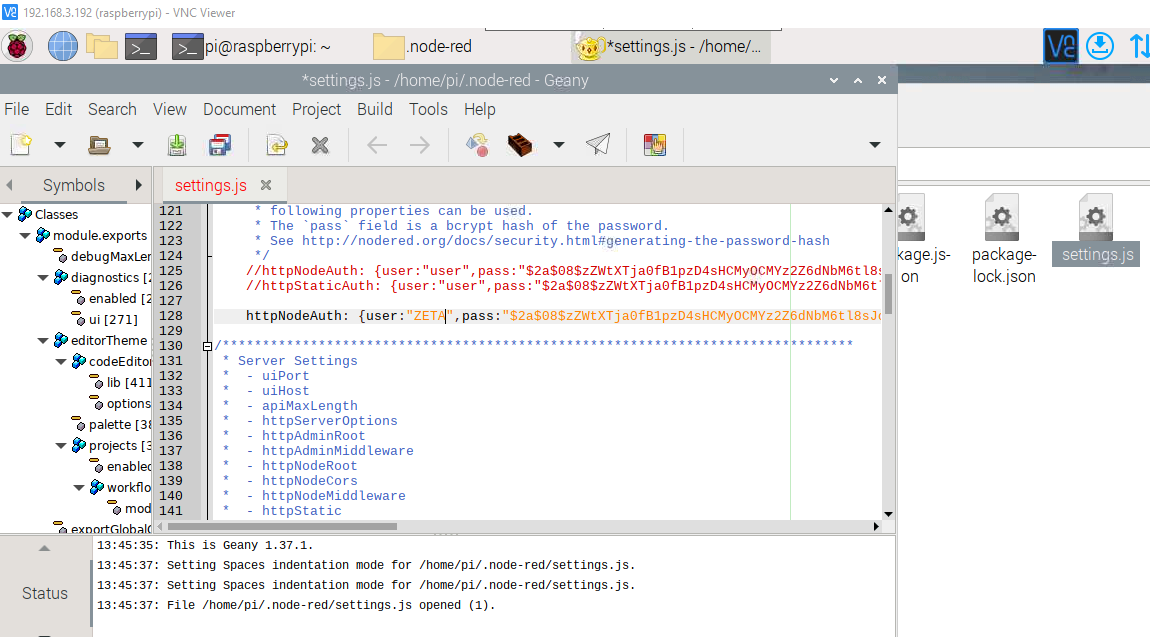
\includegraphics[width=14cm]{Images/Node-2.png}
\caption{Configuration de la sécurité dans Node-RED en Settings.js}
\label{Chap4.3.9}
\end{figure}

Dans la figure \ref{Chap4.3.9}, nous avons modifié le fichier de configuration "Settings.js" de Node-RED pour inclure des paramètres de sécurité. Cela permet de définir des utilisateurs et des mots de passe pour restreindre l'accès à notre projet.

Nous avons utilisé la commande "node-red admin hash-pw" pour générer un code de hachage sécurisé, comme le montre la figure suivante :

\begin{figure}[H]
\centering
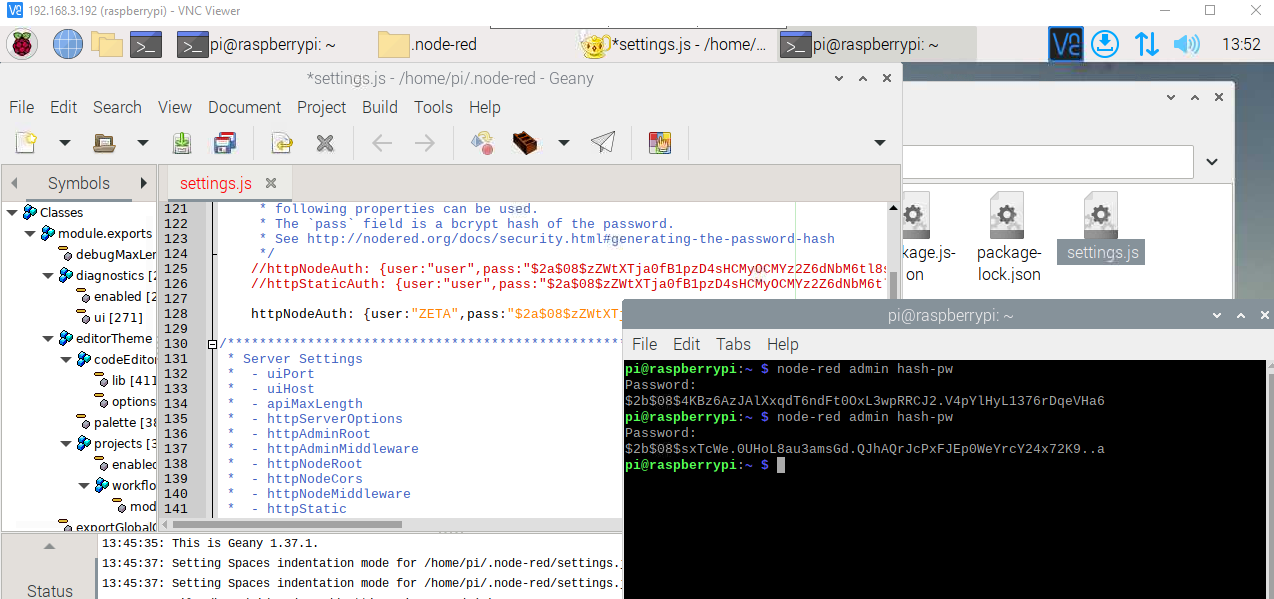
\includegraphics[width=15cm]{Images/Node-3.png}
\caption{Création d'un code de hachage}
\label{Chap4.3.10}
\end{figure}

Le code de hachage généré est ensuite ajouté au fichier "Settings.js" pour mettre à jour les informations de sécurité, comme indiqué dans la figure \ref{Chap4.3.11}.

\begin{figure}[H]
\centering
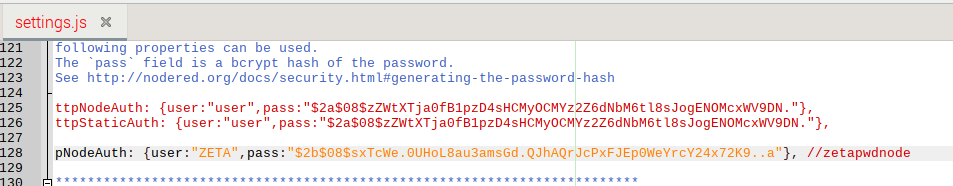
\includegraphics[width=15cm]{Images/Node-4.png}
\caption{Mise à jour du code de hachage dans Settings.js}
\label{Chap4.3.11}
\end{figure}

Une fois la sécurité configurée, nous pouvons nous connecter à Node-RED en utilisant le nouveau mot de passe, comme le montre la figure \ref{Chap4.3.12}.

\begin{figure}[H]
\centering
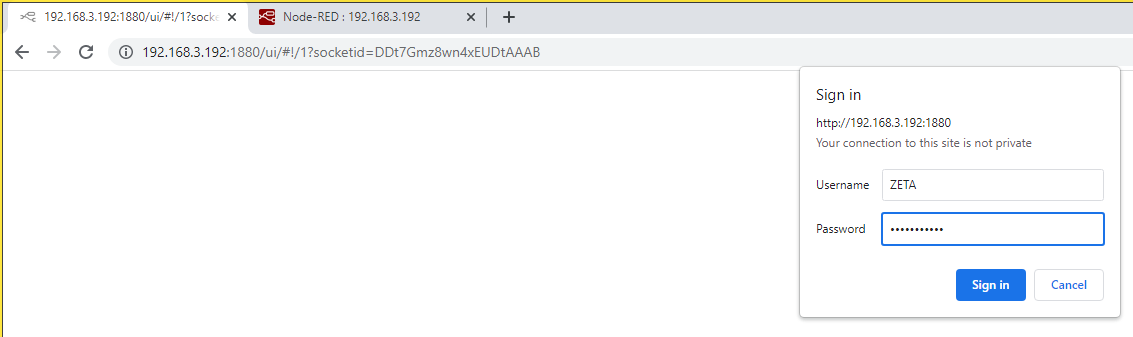
\includegraphics[width=15cm]{Images/Node-5.png}
\caption{Connexion avec le nouveau mot de passe}
\label{Chap4.3.12}
\end{figure}

Ces différentes figures décrivent le processus de sécurisation de Node-RED en utilisant des mots de passe hachés. Cela garantit que seuls les utilisateurs autorisés peuvent accéder à notre projet et protège ainsi notre système contre les accès non autorisés.
\newpage

\subsection{Réalisation en Node-RED}

Dans notre topologie, nous utilisons 2 LED, un capteur DHT11 et une breadboard, que nous avons connectés aux GPIO de Raspberry Pi, comme le montrent les figures suivantes, réalisées à l'aide de fritzing.

\begin{figure}[H]
\centering
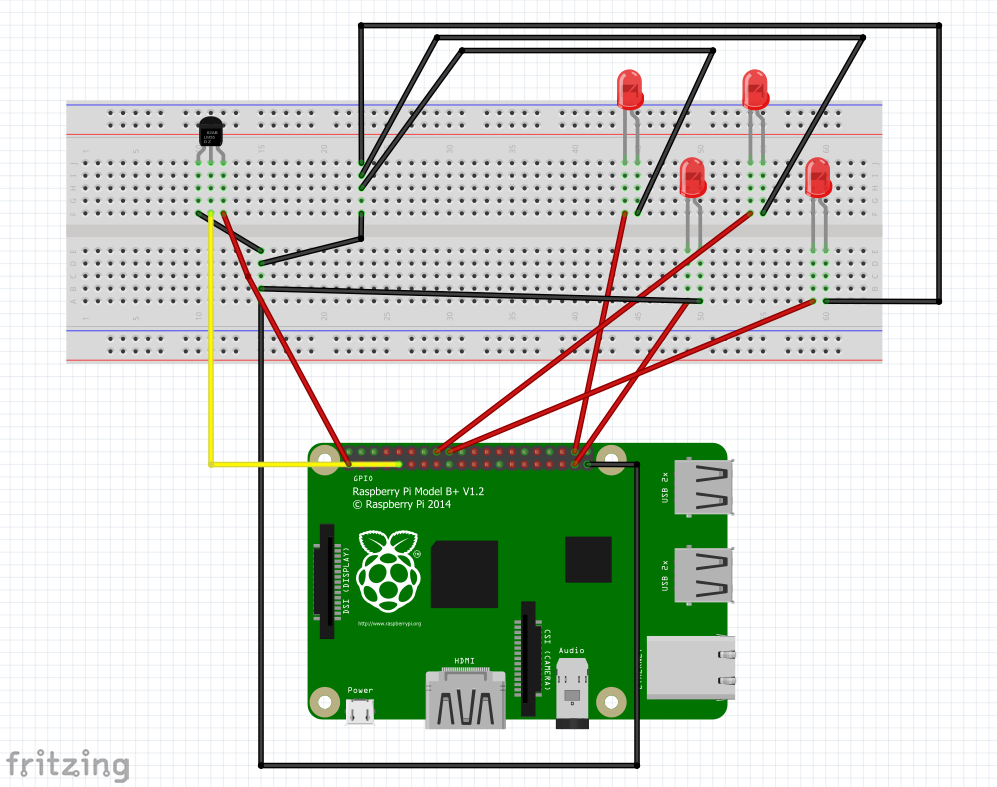
\includegraphics[width=15cm]{Images/RaspberryVisual.png}
\caption{Schéma de notre réalisation}
\label{Chap4.3.13}
\end{figure}

Dans la figure \ref{Chap4.3.13}, nous pouvons voir le schéma de notre réalisation, avec les connexions des composants sur la breadboard.

Ensuite, nous avons configuré les nodes DHT11 dans Node-RED pour séparer les données reçues entre Température et Humidité et les avons configurés pour actualiser les données toutes les 10 secondes.

\begin{figure}[H]
\centering
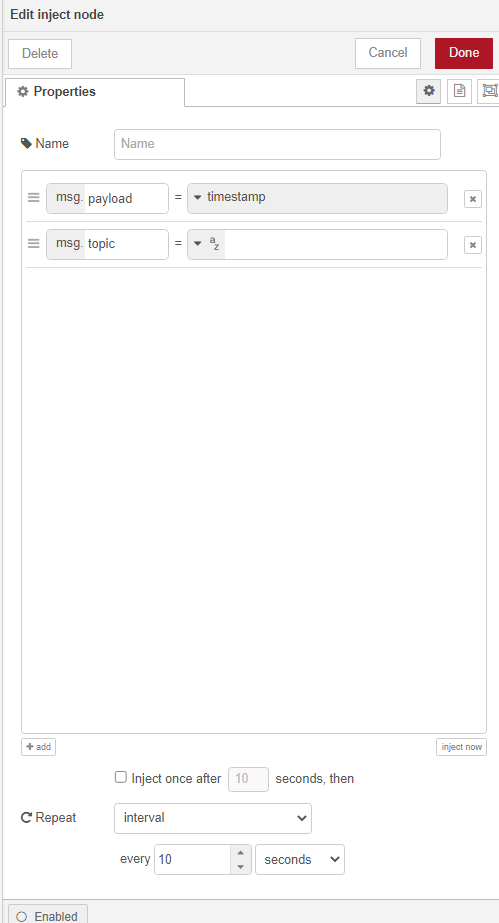
\includegraphics[width=12cm]{Images/Node-8.png}
\caption{Ajout d'un Inject Node pour répéter l'action chaque 10 secondes}
\label{Chap4.3.15}
\end{figure}

Dans la figure \ref{Chap4.3.15}, nous avons ajouté un nœud Inject pour répéter l'action toutes les 10 secondes, permettant ainsi la mise à jour régulière des données.

\begin{figure}[H]
\centering
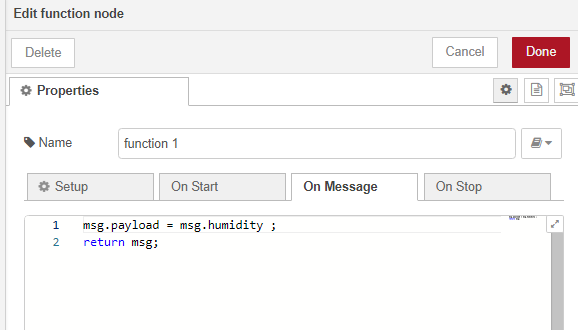
\includegraphics[width=15cm]{Images/Node-9.png}
\caption{Configurer une node Fonction pour séparer l'humidité de la température}
\label{Chap4.3.16}
\end{figure}

Dans la figure \ref{Chap4.3.16}, nous avons configuré un nœud Fonction pour séparer l'humidité de la température, ce qui permet d'obtenir des valeurs distinctes pour chaque paramètre.

\begin{figure}[H]
\centering
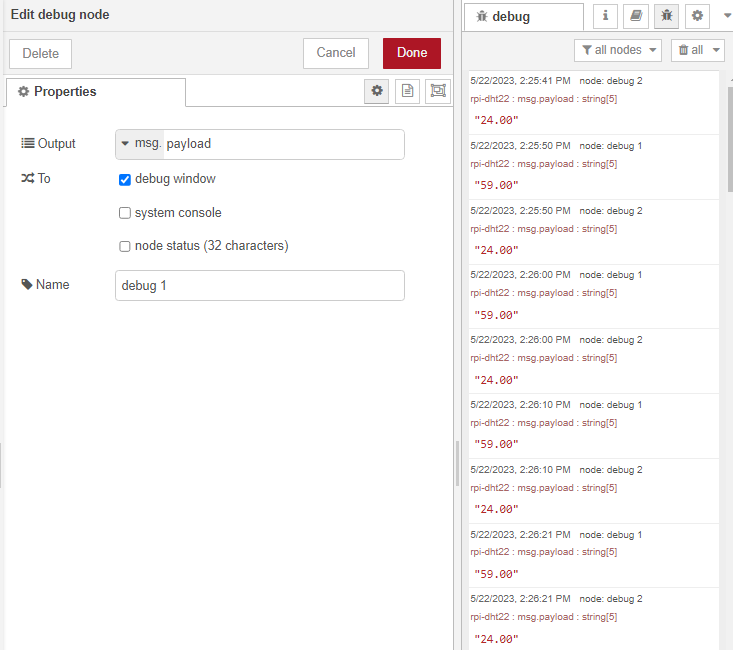
\includegraphics[width=15cm]{Images/Node-10.png}
\caption{Le résultat de Debug Node}
\label{Chap4.3.17}
\end{figure}

La figure \ref{Chap4.3.17} montre le résultat obtenu à l'aide d'un nœud Debug, où les données séparées d'humidité et de température sont affichées.

En plus, nous avons créé des nœuds pour les interrupteurs (Switches) afin de contrôler les LEDs.

\begin{figure}[H]
\centering
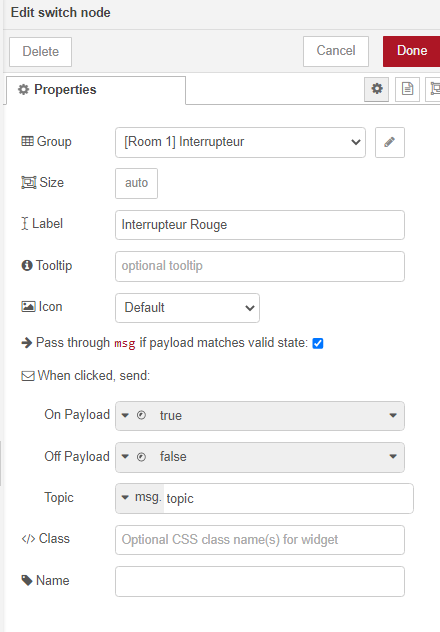
\includegraphics[width=13cm]{Images/Node-6.png}
\caption{Switch Node}
\label{Chap4.3.18}
\end{figure}

Dans la figure \ref{Chap4.3.18}, nous avons ajouté un nœud Switch pour contrôler l'état des LEDs en fonction d'une condition spécifique.

\begin{figure}[H]
\centering
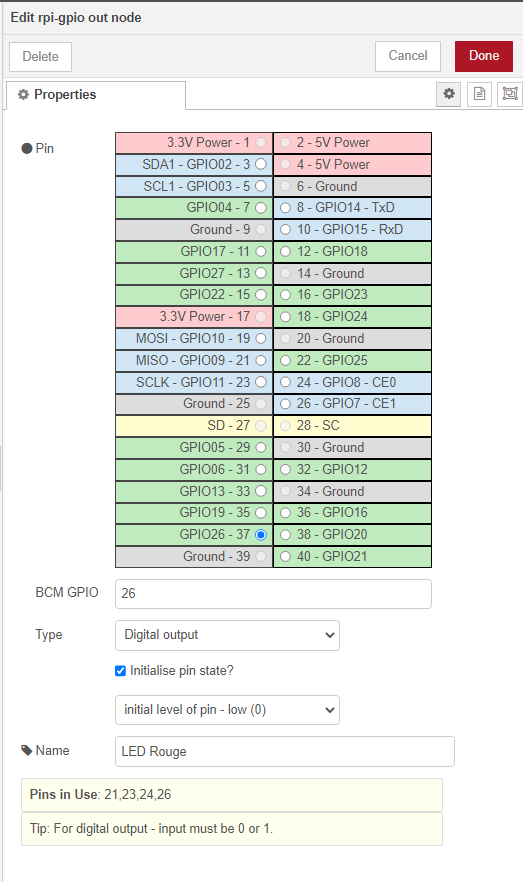
\includegraphics[width=12cm]{Images/Node-7.png}
\caption{Raspberry GPIO Output Node}
\label{Chap4.3.19}
\end{figure}

La figure \ref{Chap4.3.19} présente le nœud Raspberry GPIO Output utilisé pour contrôler les GPIO du Raspberry Pi et allumer/éteindre les LEDs.

Et enfin, voici les

 nœuds et l'exécution finale de mon projet Node-RED.

\begin{figure}[H]
\centering
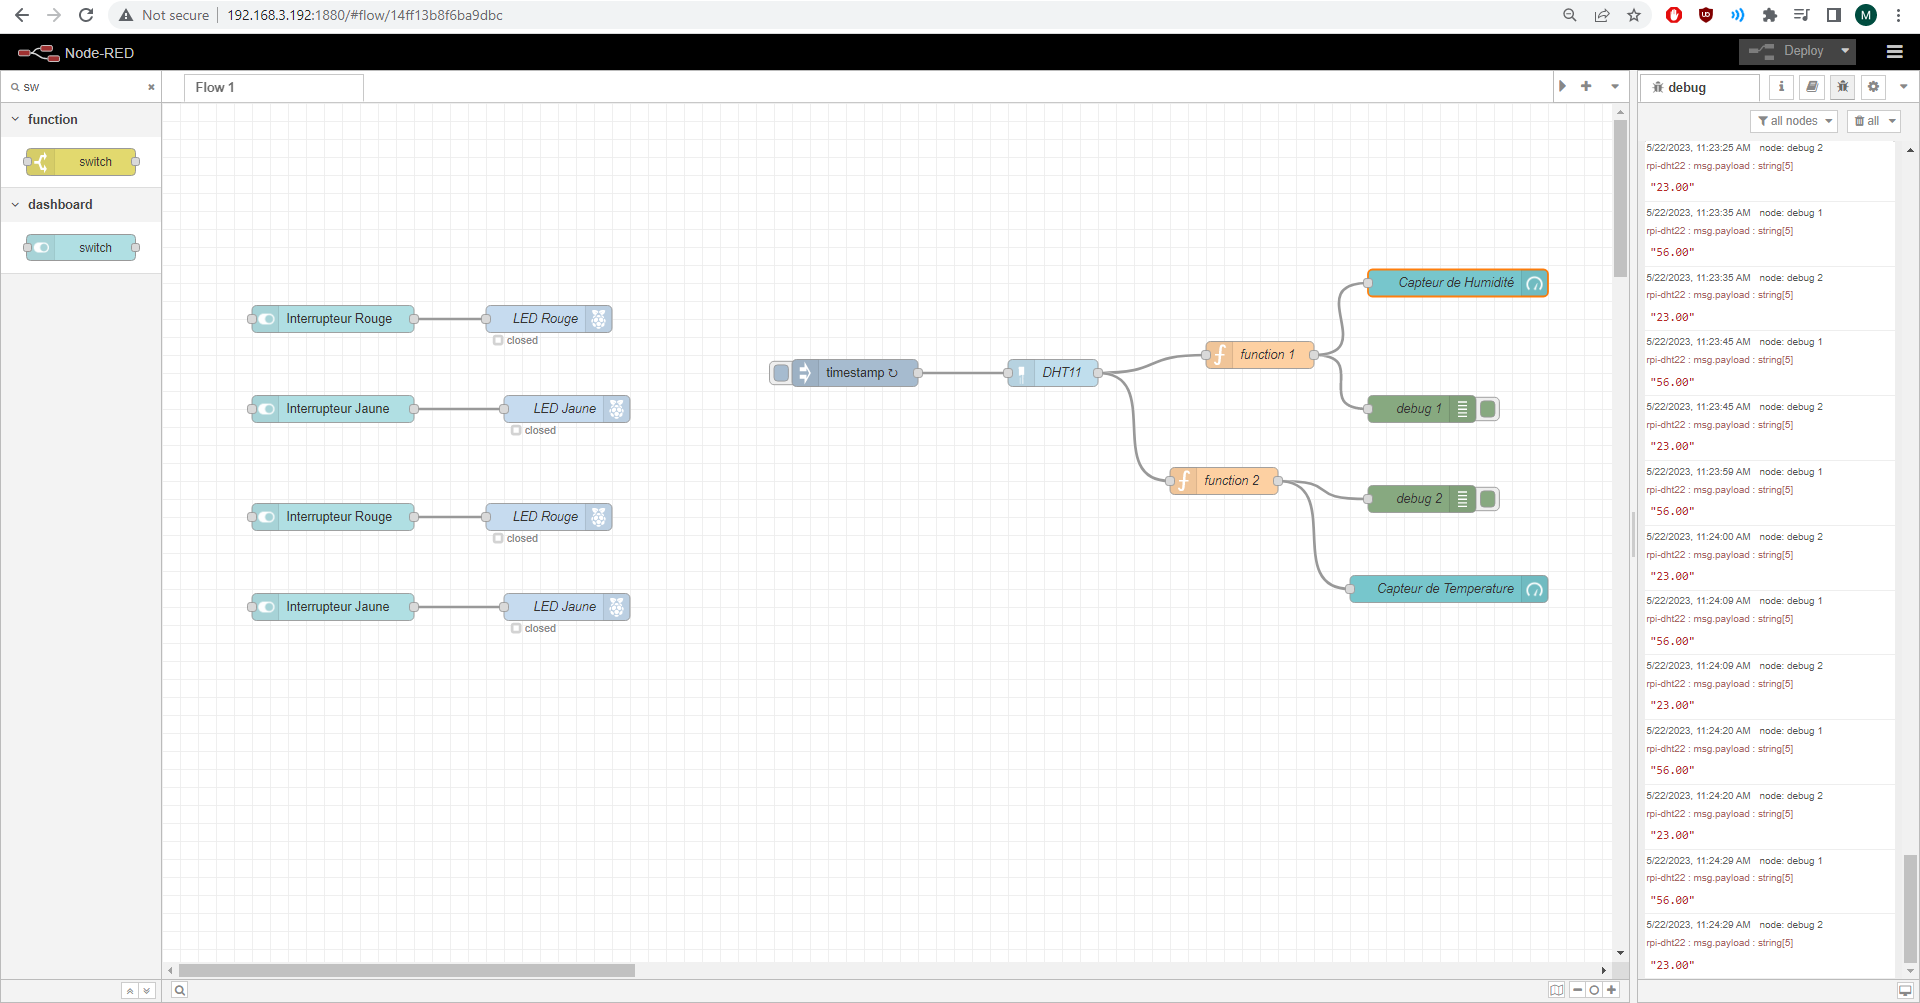
\includegraphics[width=15cm]{Images/Node-1.png}
\caption{Le Projet en Node-RED}
\label{Chap4.3.20}
\end{figure}

La figure \ref{Chap4.3.20} présente le projet Node-RED complet avec tous les nœuds configurés et connectés.

\begin{figure}[H]
\centering
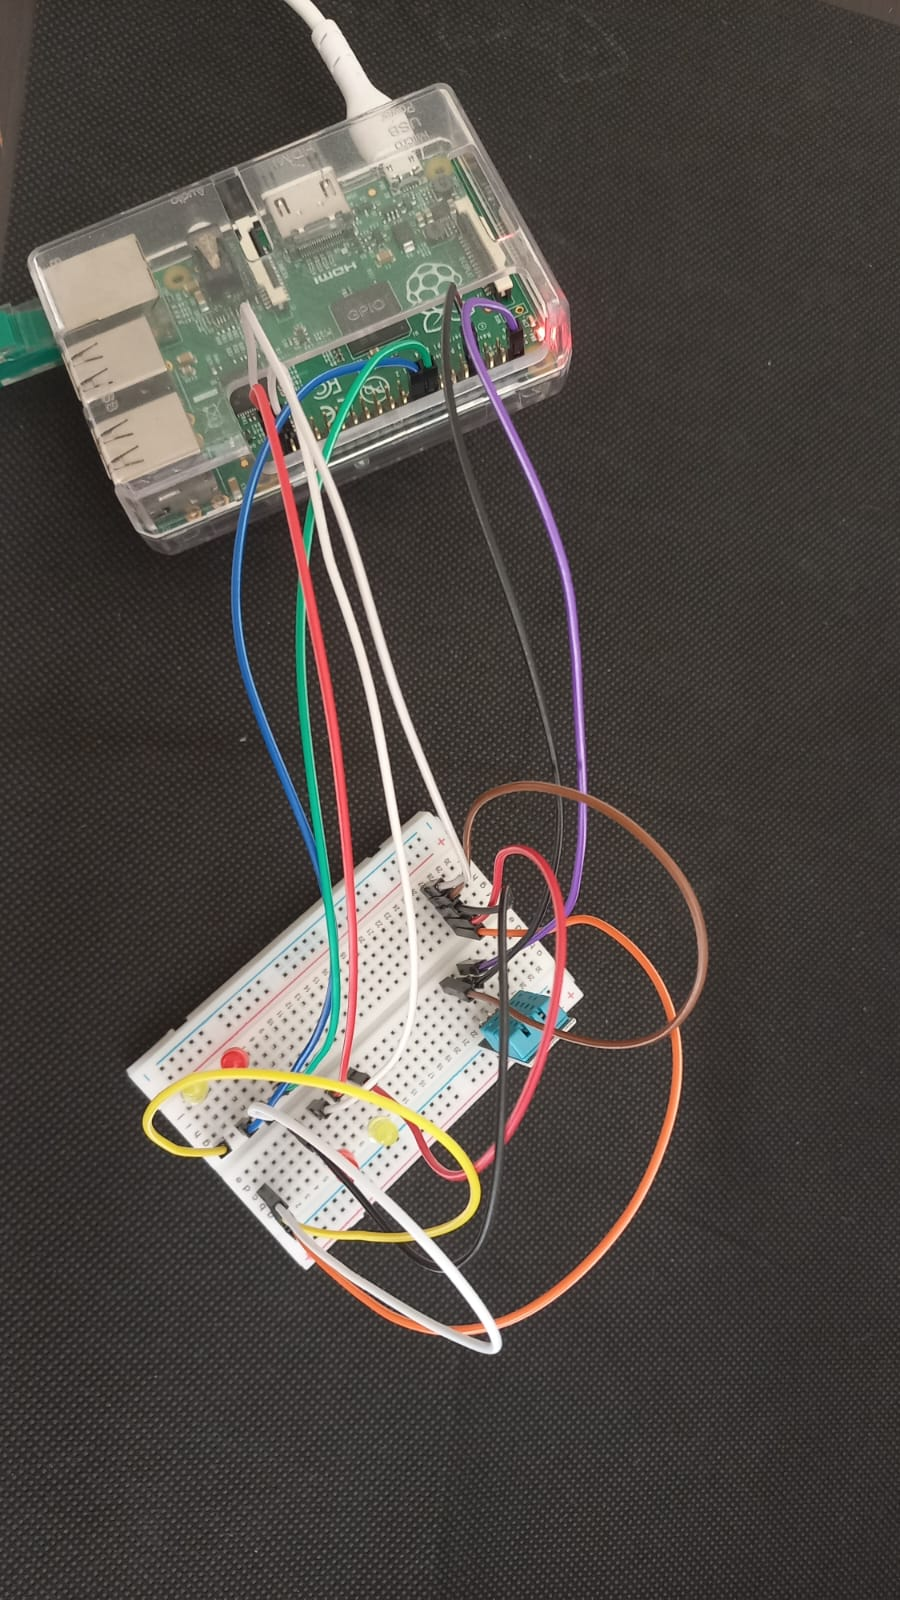
\includegraphics[width=10cm]{Images/Node-11.jpg}
\caption{Circuit de mon Projet}
\label{Chap4.3.21}
\end{figure}

Dans la figure \ref{Chap4.3.21}, nous pouvons voir le circuit physique de notre projet, avec les composants connectés sur la breadboard et le Raspberry Pi.

\begin{figure}[H]
\centering
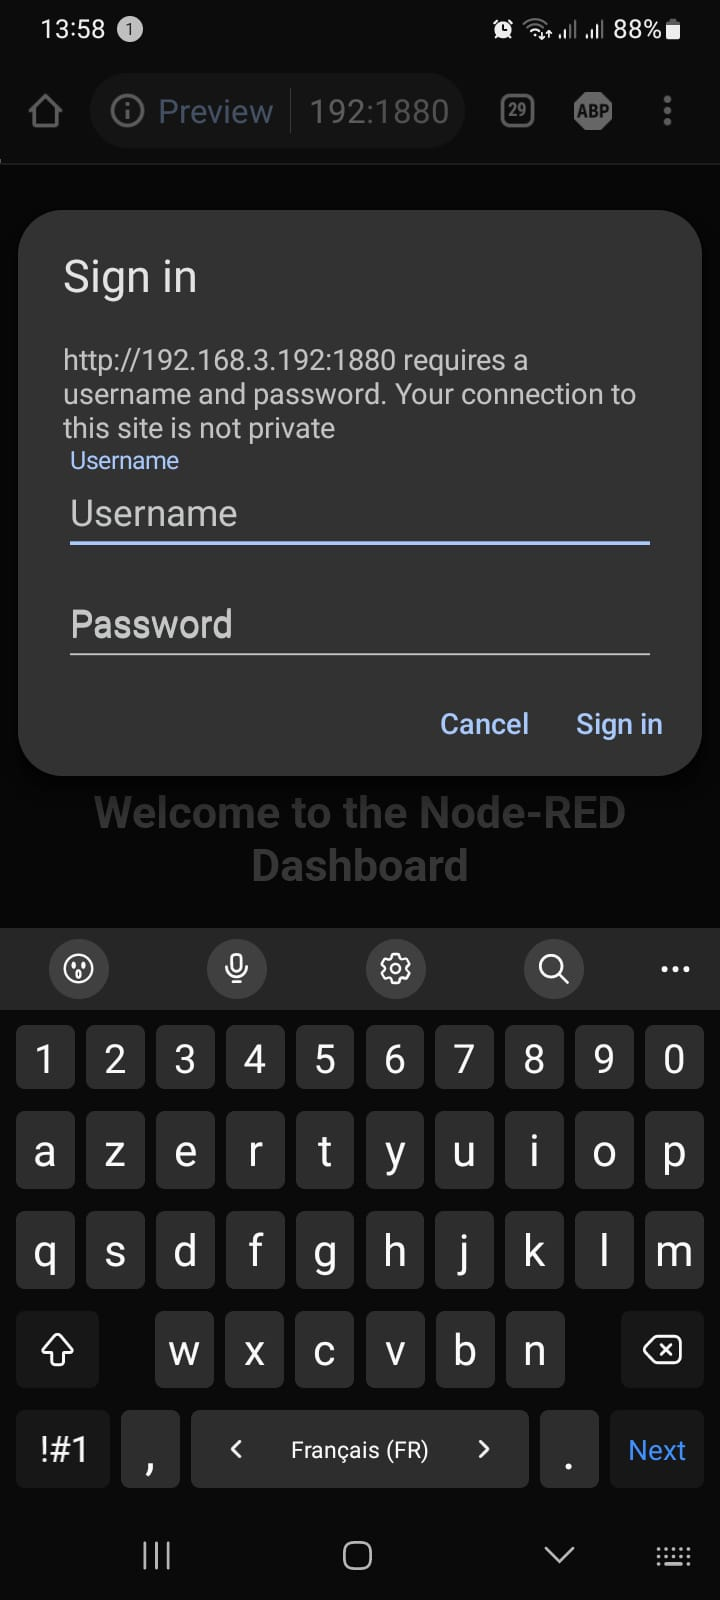
\includegraphics[width=10cm]{Images/1006591.jpg}
\caption{Le Dashboard Login en Mobile}
\label{Chap4.3.22}
\end{figure}

La figure \ref{Chap4.3.22} présente l'interface de connexion (Dashboard Login) de notre projet, adaptée pour une utilisation sur mobile.

\begin{figure}[H]
\centering
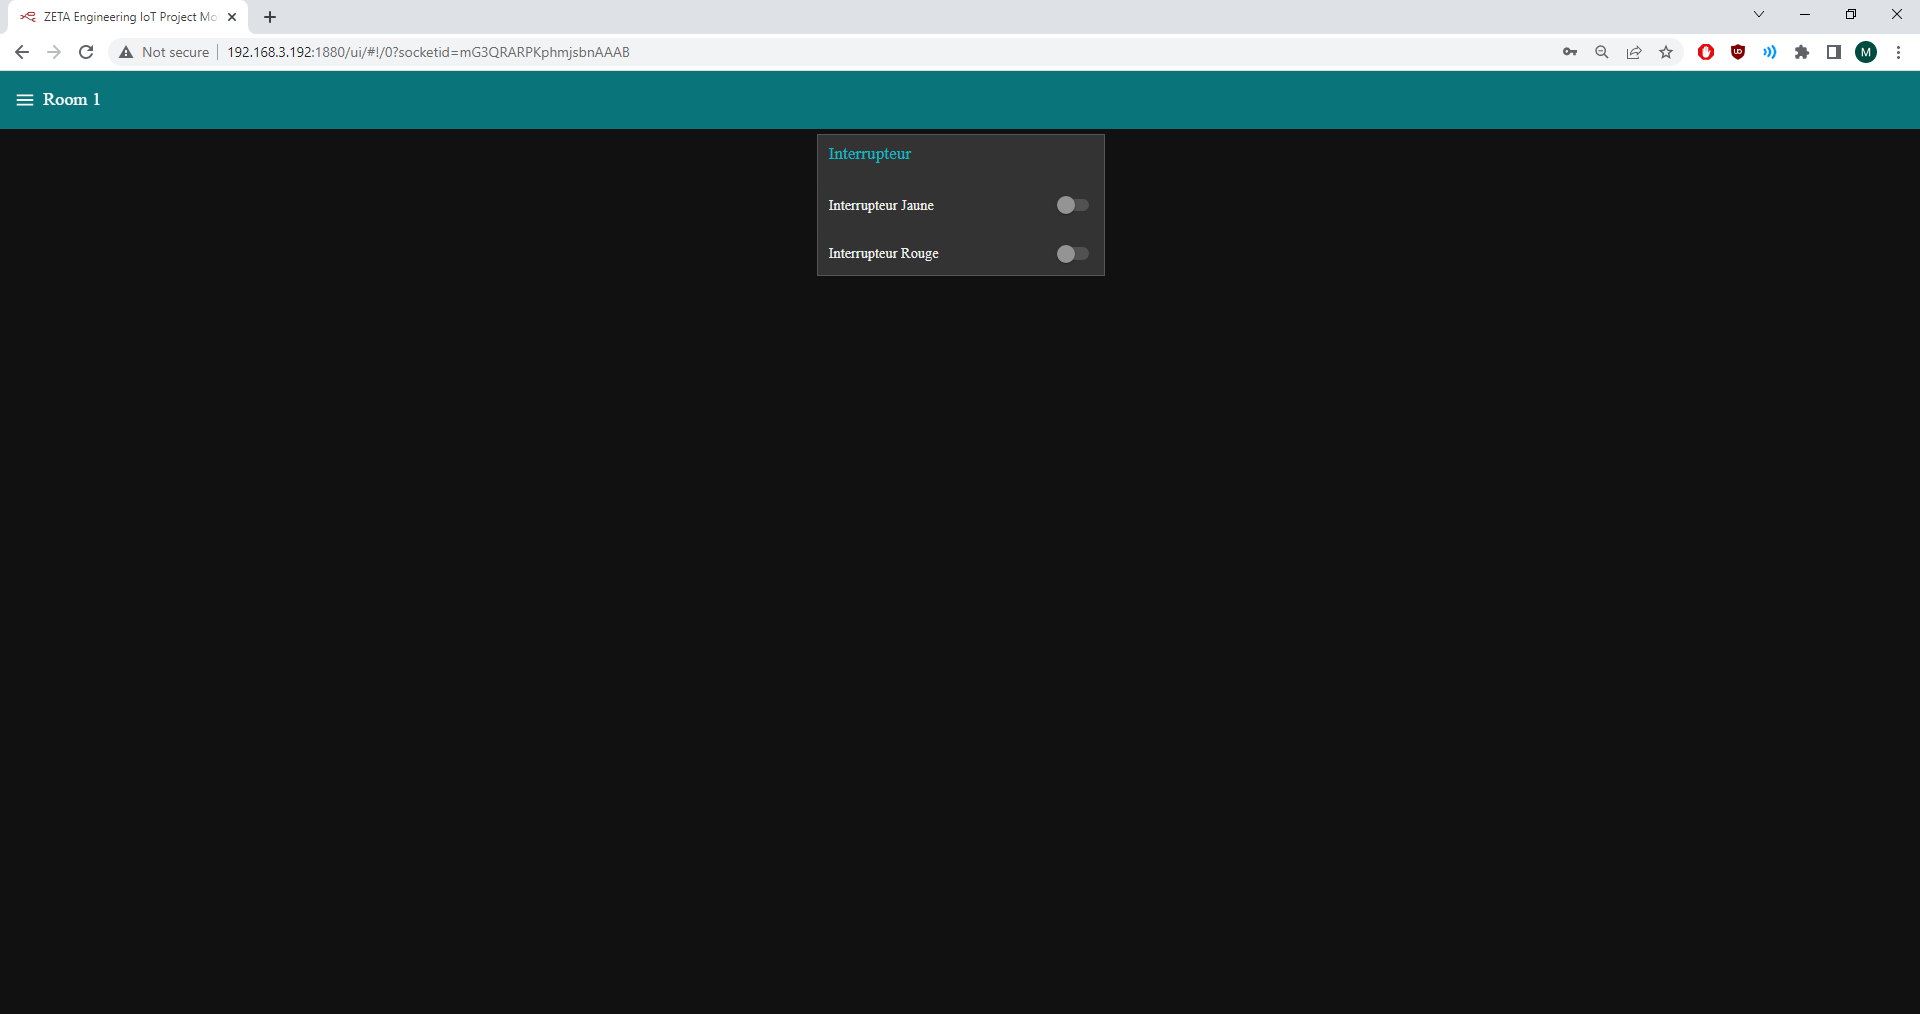
\includegraphics[width=13cm]{Images/150131.png}
\caption{Le Dashboard Room 1 en Chrome}
\label{Chap4.3.23}
\end{figure}

La figure \ref{Chap4.3.23} montre le tableau de bord (Dashboard) de la salle 1 de notre projet, affiché dans le navigateur Chrome.

\begin{figure}[H]
\centering
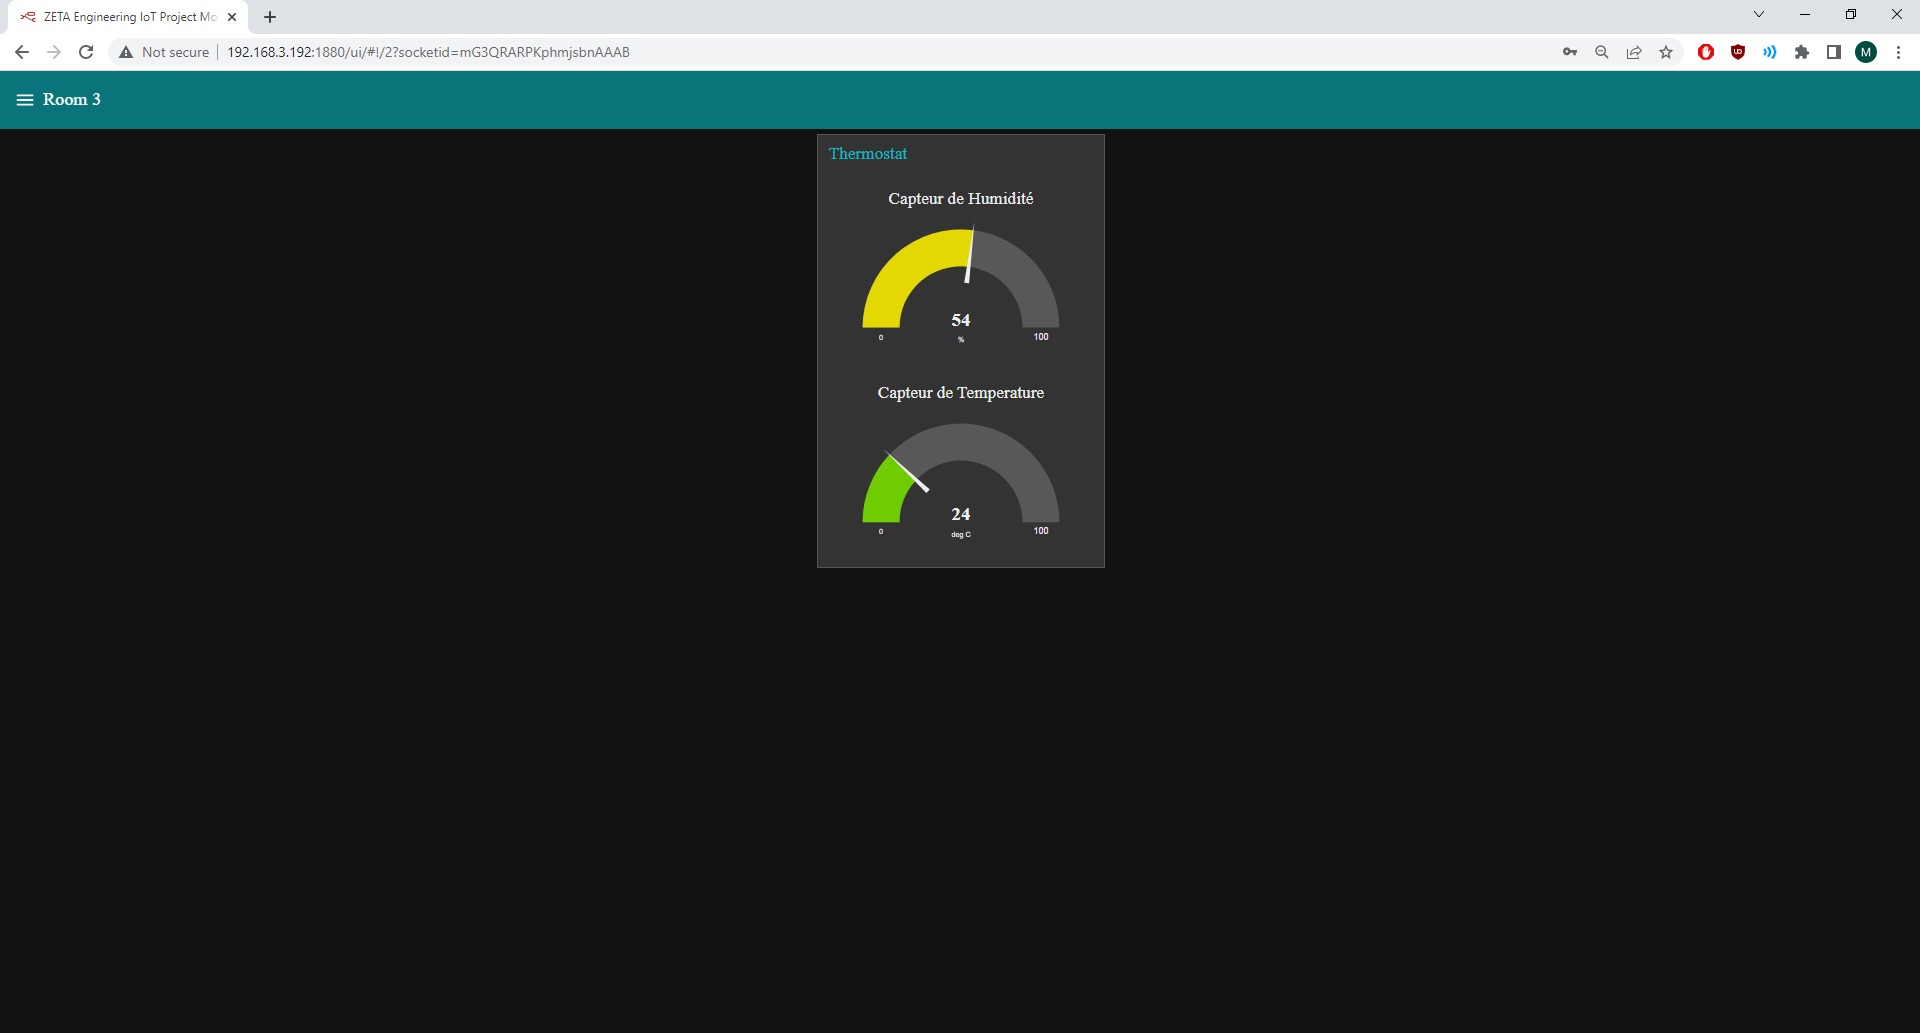
\includegraphics[width=13cm]{Images/150156.png}
\caption{Le Dashboard Room 3 en Chrome}
\label{Chap4.3.24}
\end{figure}

Dans la figure \ref{Chap4.3.24}, nous pouvons voir le tableau de bord (Dashboard) de la salle 3 de notre projet, également affiché dans le navigateur Chrome.

\begin{figure}[H]
\centering
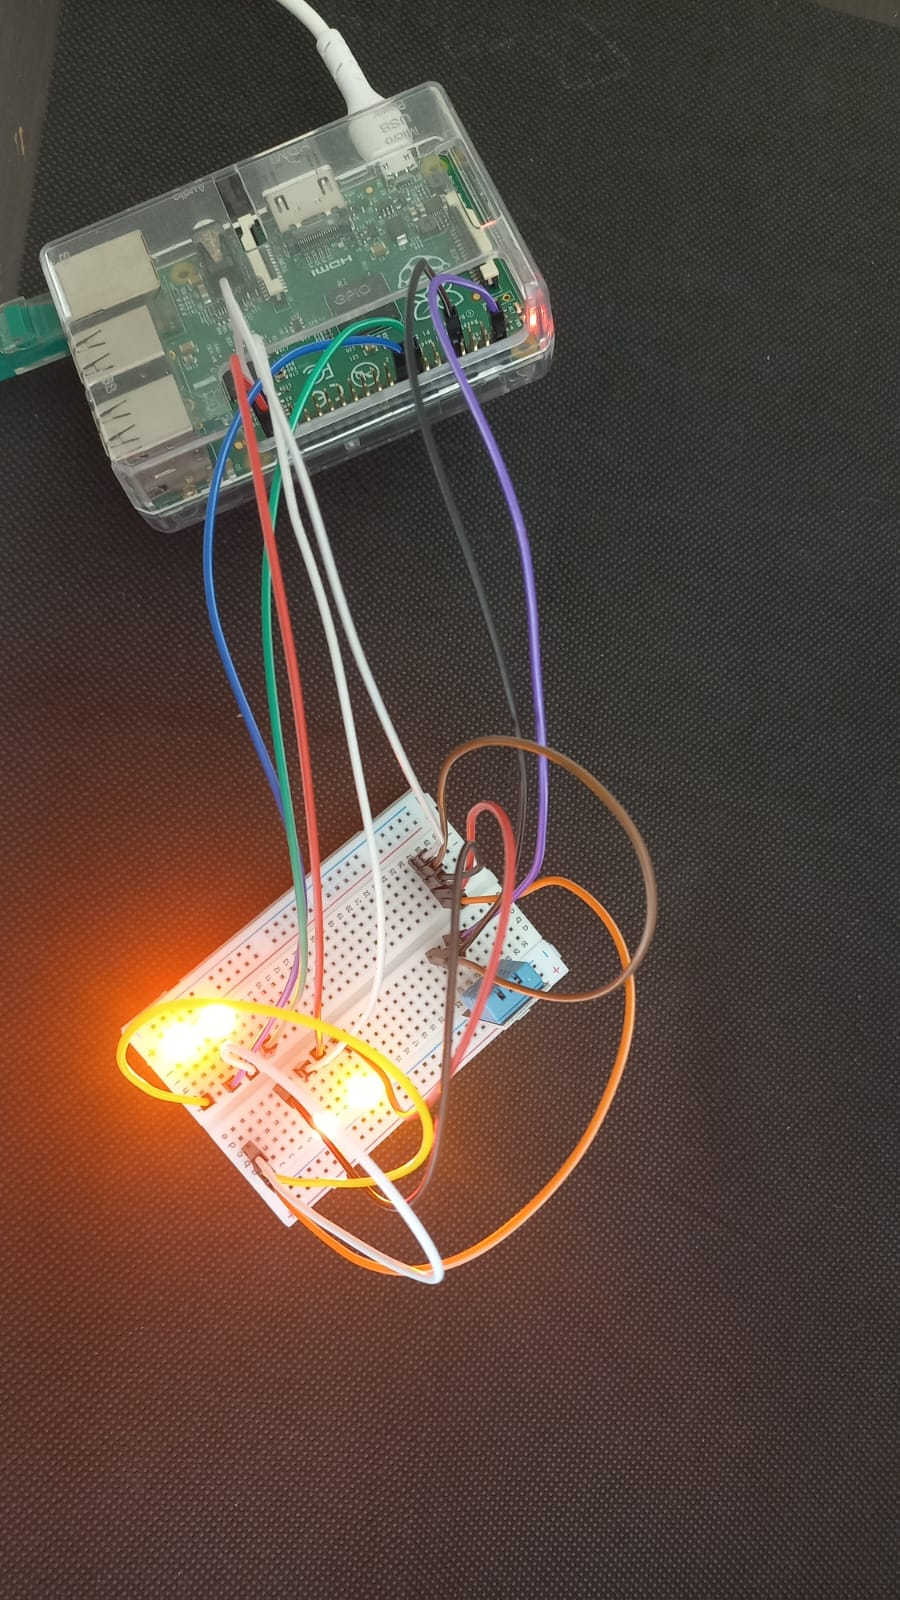
\includegraphics[width=10cm]{Images/Node-12.jpg}
\caption{Circuit de mon Projet en marche}
\label{Chap4.3.25}
\end{figure}

Enfin, la figure \ref{Chap4.3.25} illustre le circuit de notre projet en pleine exécution, avec les LEDs allumées et les données d'humidité et de température affichées sur le tableau de bord.

Ces différentes figures témoignent de notre réalisation en Node-RED et illustrent les différentes étapes et résultats obtenus dans notre projet.


\subsection{Intégration dans le parc informatique}

Une fois notre application prête, nous pouvons l'intégrer dans le parc informatique que nous avons créé dans le troisième chapitre à l'aide de GLPI.

Pour cela, nous avons installé le FusionInventory-Agent sur notre Raspberry Pi, comme illustré ci-dessous :

\begin{figure}[H]
\centering
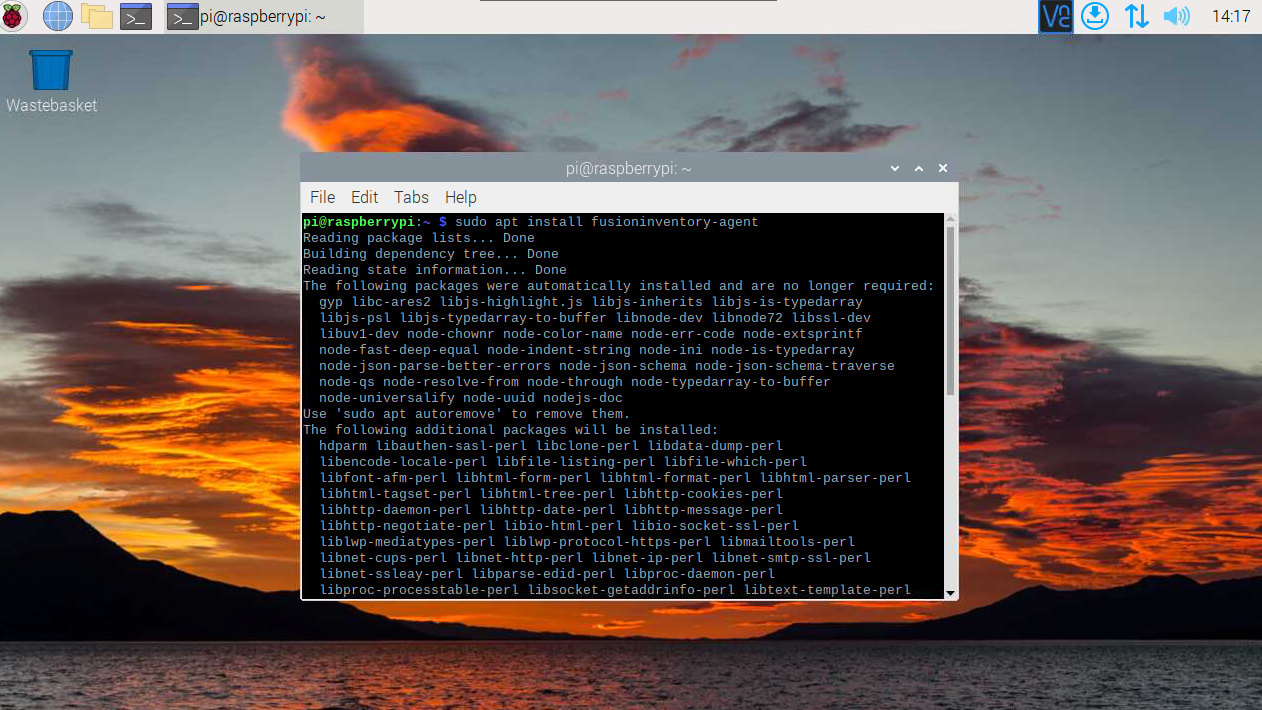
\includegraphics[width=15cm]{Images/raspberryfusion.png}
\caption{Installation de FusionInventory-Agent}
\label{fig:raspberry-fusion}
\end{figure}

Ensuite, nous avons configuré le FusionInventory-Agent pour qu'il envoie les données de notre périphérique au serveur GLPI à l'adresse "192.168.3.66/glpi/fusioninventory", comme présenté dans la figure suivante :

\begin{figure}[H]
\centering
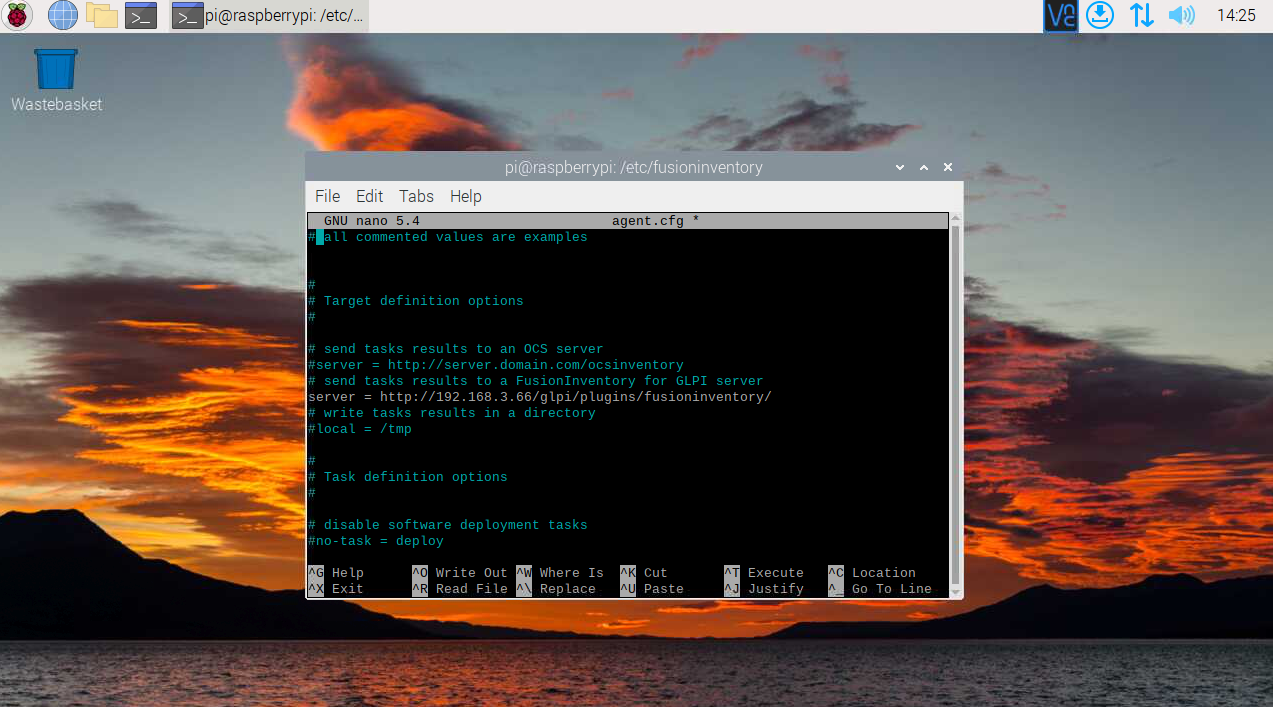
\includegraphics[width=15cm]{Images/raspberryfusion1.png}
\caption{Configuration de FusionInventory-Agent}
\label{fig:raspberry-fusion-config}
\end{figure}

Enfin, nous pouvons visualiser notre Raspberry Pi intégré dans le tableau de bord de GLPI :

\begin{figure}[H]
\centering
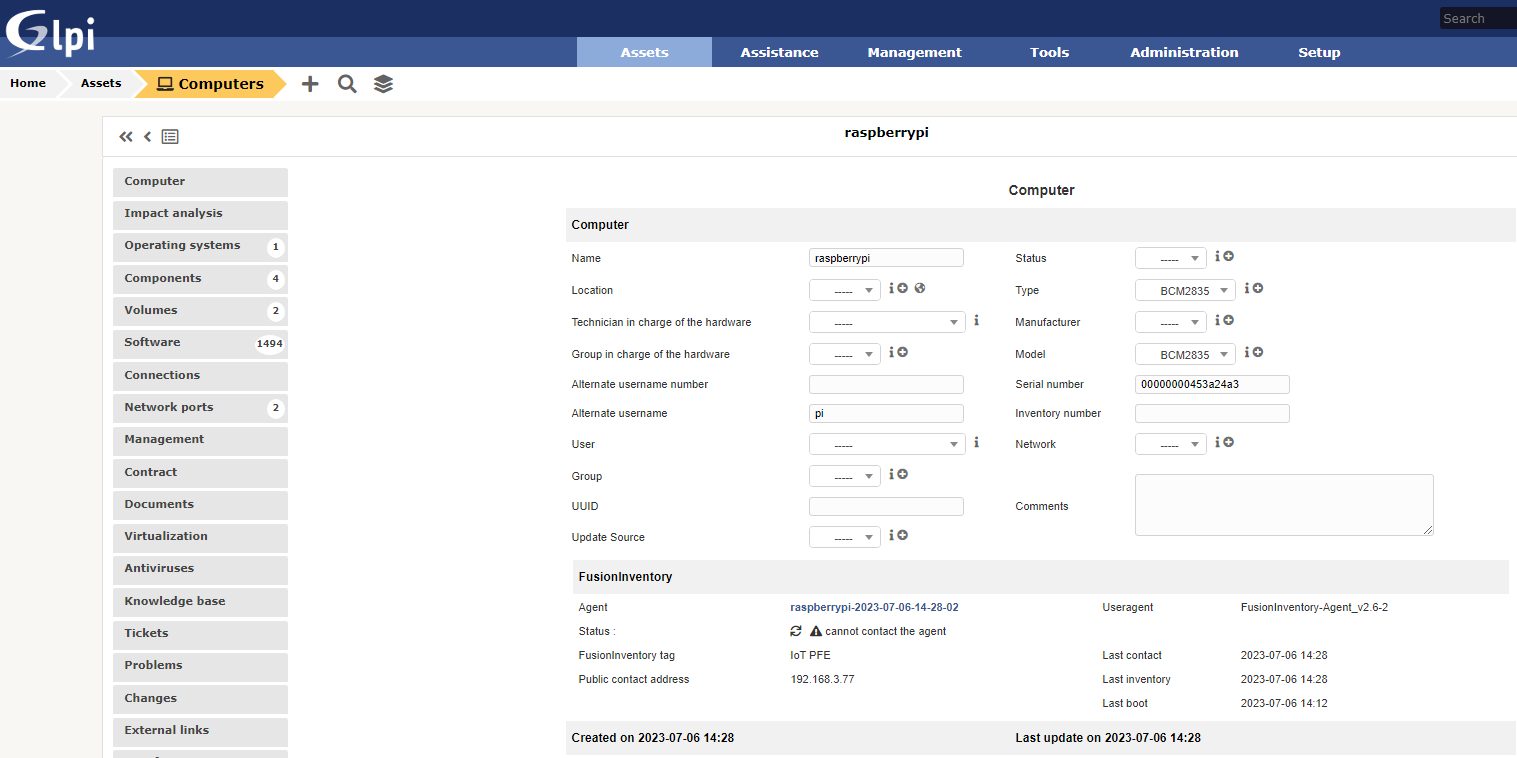
\includegraphics[width=15cm]{Images/RASPBERRYPIGLPI.png}
\caption{Tableau de bord de GLPI avec le Raspberry Pi intégré}
\label{fig:glpi-raspberry}
\end{figure}

\section{Conclusion}


En conclusion de ce chapitre sur l'intégration des objets connectés dans l'infrastructure informatique de l'entreprise, nous avons vu que cette étape est cruciale pour permettre une gestion intelligente et à distance des différents équipements de la société. Nous avons utilisé des cartes IoT telles que Raspberry Pi pour connecter les différents objets tels que les lampes et les machines de pointage au réseau de l'entreprise. Nous avons également utilisé des logiciels tels que ZKAccess et SmartPSS pour contrôler ces objets à distance. \\

Les objets connectés sont de plus en plus présents dans notre vie quotidienne, que ce soit dans les maisons, les voitures ou les entreprises. Les chiffres montrent que le marché de l'IoT devrait continuer à croître de manière significative dans les années à venir. L'intégration de ces objets dans l'infrastructure informatique de l'entreprise permet une gestion plus efficace et une prise de décision plus éclairée grâce à la collecte de données en temps réel. \\

En somme, l'intégration des objets connectés dans l'infrastructure informatique de l'entreprise apporte de nombreux avantages en termes de gestion, de prise de décision et d'efficacité. Cependant, il est important de prendre en compte les aspects de sécurité et de protection des données pour garantir une utilisation sûre et efficace de ces objets. \\




